\section{Khảo sát thực tế}

\subsection{Thực trạng các giao thức nhắn tin mã hóa đầu cuối}

Sự phổ biến của các ứng dụng nhắn tin trực tuyến đã kéo theo nhu cầu ngày càng cao về bảo vệ quyền riêng tư và tính bảo mật của dữ liệu trao đổi. Để đáp ứng yêu cầu đó, mã hóa đầu cuối (End-to-End Encryption - E2EE) đã trở thành cơ chế bảo mật cốt lõi trong nhiều nền tảng nhắn tin hiện đại. Với E2EE, nội dung tin nhắn được mã hóa tại thiết bị người gửi và chỉ được giải mã tại thiết bị người nhận, giúp ngăn chặn việc đọc trộm dữ liệu bởi máy chủ trung gian hoặc các bên thứ ba.

Hiện nay, nhiều ứng dụng nhắn tin phổ biến đã triển khai E2EE dưới các hình thức khác nhau. Trong đó, Signal được xem là một trong những nền tảng tiên phong với Signal Protocol, giao thức đã trở thành cơ sở cho cơ chế bảo mật của WhatsApp, Google Messages và nhiều hệ thống liên lạc khác. Các giao thức này không chỉ cung cấp tính bí mật của nội dung trao đổi mà còn hỗ trợ các thuộc tính an toàn quan trọng như xác thực người dùng, bí mật chuyển tiếp (Forward Secrecy) và bí mật hậu thỏa hiệp (Post-Compromise Security).

Bên cạnh việc bảo vệ nội dung tin nhắn, các giao thức hiện đại còn phải giải quyết nhiều yêu cầu phức tạp hơn như đồng bộ trên nhiều thiết bị, hỗ trợ người dùng ngoại tuyến, quản lý khóa phiên động và đảm bảo hiệu năng khi số lượng người dùng tăng cao. Điều này khiến thiết kế giao thức nhắn tin trở thành một bài toán tổng hợp giữa mật mã học, kiến trúc hệ thống và trải nghiệm người dùng.

\subsection{Các cơ chế bảo mật được sử dụng trong hệ thống nhắn tin hiện nay}

Phần lớn các hệ thống E2EE hiện nay áp dụng mô hình mật mã lai (Hybrid Cryptography), trong đó mật mã khóa công khai được sử dụng để thiết lập khóa phiên và mật mã đối xứng được sử dụng để mã hóa dữ liệu thực tế.

Trong Signal Protocol, quá trình thiết lập khóa ban đầu được thực hiện thông qua Extended Triple Diffie-Hellman (X3DH), cho phép hai người dùng tạo khóa chung ngay cả khi một bên đang ngoại tuyến. Sau khi khóa ban đầu được thiết lập, cơ chế Double Ratchet được sử dụng để liên tục cập nhật khóa phiên sau mỗi lần trao đổi tin nhắn. Nhờ đó, việc lộ khóa ở một thời điểm không làm ảnh hưởng đến toàn bộ lịch sử liên lạc.

Mô hình này đã chứng minh được hiệu quả trong thực tế và hiện được xem là tiêu chuẩn tham chiếu cho việc xây dựng các ứng dụng nhắn tin bảo mật. Tuy nhiên, nền tảng trao đổi khóa của các giao thức này vẫn chủ yếu dựa trên mật mã đường cong elliptic, vốn được thiết kế cho môi trường tính toán cổ điển.

\subsection{Những thách thức trong thiết kế giao thức nhắn tin thế hệ mới}

Mặc dù các giao thức hiện nay đã đạt được mức độ bảo mật cao, việc thiết kế một hệ thống nhắn tin an toàn vẫn còn nhiều thách thức.

Thứ nhất, hệ thống phải duy trì các thuộc tính an toàn cốt lõi như tính bí mật, tính toàn vẹn, xác thực, bí mật chuyển tiếp và khả năng phục hồi sau khi khóa bị lộ. Đây là những yêu cầu bắt buộc đối với các ứng dụng nhắn tin hiện đại.

Thứ hai, giao thức cần đảm bảo khả năng hoạt động hiệu quả trong môi trường thực tế với độ trễ thấp, tiêu tốn ít tài nguyên và có khả năng mở rộng cho số lượng lớn người dùng.

Thứ ba, sự phát triển của điện toán lượng tử đặt ra yêu cầu phải xem xét lại các cơ chế trao đổi khóa đang được sử dụng. Mặc dù các giao thức hiện tại vẫn được đánh giá là an toàn trước các phương thức tấn công truyền thống, việc chuẩn bị cho quá trình chuyển đổi sang các thuật toán kháng lượng tử đang trở thành xu hướng nghiên cứu và phát triển quan trọng trong lĩnh vực bảo mật truyền thông.

\subsection{Xu hướng tích hợp mật mã hậu lượng tử vào hệ thống nhắn tin}

Sau khi các tiêu chuẩn mật mã hậu lượng tử được công bố, nhiều tổ chức nghiên cứu và doanh nghiệp công nghệ đã bắt đầu thử nghiệm việc tích hợp các thuật toán hậu lượng tử vào các giao thức truyền thông hiện có. Thay vì thay thế hoàn toàn các cơ chế hiện hữu, phần lớn giải pháp được đề xuất theo hướng hybrid, kết hợp đồng thời thuật toán truyền thống và thuật toán hậu lượng tử trong quá trình trao đổi khóa.

Cách tiếp cận này cho phép hệ thống duy trì khả năng tương thích với các nền tảng hiện tại trong khi từng bước nâng cao khả năng chống chịu trước các mối đe dọa trong tương lai. Tuy nhiên, việc tích hợp mật mã hậu lượng tử cũng làm phát sinh nhiều vấn đề cần nghiên cứu như kích thước khóa lớn hơn, chi phí truyền thông tăng lên và ảnh hưởng đến hiệu năng của giao thức.

Từ thực trạng trên có thể thấy rằng việc xây dựng một giao thức nhắn tin mã hóa đầu cuối kết hợp các cơ chế bảo mật hiện đại với giải pháp trao đổi khóa kháng lượng tử là hướng nghiên cứu có ý nghĩa cả về mặt học thuật lẫn thực tiễn.

\section{Phân tích yêu cầu hệ thống}

\subsection{Mục tiêu chức năng và phi chức năng}

\textbf{Yêu cầu chức năng}

\begin{itemize}
    \item \textbf{Quản lý tài khoản:} đăng ký, đăng nhập, đổi mật khẩu, quản lý hồ sơ cá nhân, thiết lập quyền riêng tư và chính sách cache cục bộ.

    \item \textbf{Quản lý quan hệ bạn bè:} tìm kiếm người dùng, gửi lời mời kết bạn, chấp nhận, từ chối, xóa bạn và chặn người dùng.

    \item \textbf{Nhắn tin trực tiếp E2EE:} thiết lập phiên liên lạc an toàn, gửi và nhận tin nhắn được bảo vệ bằng mã hóa đầu cuối.

    \item \textbf{Quản lý tin nhắn:} hỗ trợ trả lời, chỉnh sửa, ghim, chuyển tiếp, xóa và thả cảm xúc cho tin nhắn.

    \item \textbf{Tùy chọn hội thoại:} tắt thông báo, lưu trữ, ghim hội thoại và đánh dấu chưa đọc.

    \item \textbf{Gửi và nhận tệp tin:} hỗ trợ chia sẻ tệp đính kèm trong các cuộc trò chuyện, preview ảnh.

    \item \textbf{Hội thoại nhóm MLS:} tạo nhóm, quản lý thành viên và trao đổi tin nhắn nhóm bằng giao thức MLS.

    \item \textbf{Kiểm tra danh tính và bảo mật:} xác minh identity key qua safety number, xoay khóa an toàn (rotate identity) và theo dõi trạng thái bảo mật của cuộc trò chuyện và nhóm.

    \item \textbf{Sao lưu và khôi phục E2EE:} xuất và phục hồi dữ liệu mã hóa trên thiết bị khác.

\end{itemize}

\textbf{Yêu cầu phi chức năng}

\begin{itemize}
    \item \textbf{Giao diện người dùng:} giao diện trực quan, dễ sử dụng đối với người dùng desktop.

    \item \textbf{Hiệu năng:} phản hồi nhanh khi gửi tin nhắn, tải lịch sử và chuyển đổi hội thoại.

    \item \textbf{Bảo mật:} đảm bảo tính bí mật, toàn vẹn và xác thực của dữ liệu trao đổi với các thuộc tính: kháng lượng tử, forward secrecy, server không đọc được plaintext.

    \item \textbf{Khả năng mở rộng:} dễ dàng bổ sung chức năng hoặc nâng cấp hệ thống trong tương lai.

    \item \textbf{Tính ổn định:} hệ thống hoạt động ổn định và có khả năng phục hồi khi xảy ra lỗi.

    \item \textbf{Tính khả dụng:} có health/readiness check và metrics để giám sát trạng thái vận hành.

    \item \textbf{Tương thích đa nền tảng:} client PyQt chạy trên Windows, Linux và macOS từ cùng một mã nguồn.

\end{itemize}

\subsection{Đối tượng sử dụng và kịch bản sử dụng chính}

\begin{table}[H]
    \centering
    \small
    \begin{tabularx}{\linewidth}{|p{0.22\linewidth}|p{0.18\linewidth}|X|}
        \hline
        \textbf{Tác nhân} & \textbf{Loại} & \textbf{Vai trò} \\
        \hline
        Người dùng & Chính & Đăng ký, đăng nhập, kết bạn, nhắn tin, tạo group, kiểm tra identity, quản lý backup và quyền riêng tư. \\
        \hline
        Quản trị vận hành & Phụ & Khởi động Docker, quan sát health, metrics, log, reset dữ liệu demo và kiểm tra trạng thái server. \\
        \hline
        Auditor & Phụ & Dựng checkpoint từ identity log và cung cấp proof cho client. \\
        \hline
    \end{tabularx}
    \caption{Actor và vai trò}
    \label{tab:actors}
\end{table}

\subsection{Danh sách Use Case mức hệ thống}

Ở mức hệ thống, các chức năng của SecChat được chia thành sáu nhóm Use Case, gắn với ba tác nhân đã nêu ở bảng~\ref{tab:actors}.

\begin{itemize}
  \item \textbf{Nhóm A: Quản lý tài khoản và danh tính}\\
  Các chức năng khởi tạo tài khoản, xác thực và quản lý danh tính bảo mật của người dùng.
  \begin{itemize}
    \item \textbf{Đăng ký (UC01):} tạo tài khoản bằng username, email và mật khẩu; client khởi tạo state E2EE và công bố khóa lần đầu.
    \item \textbf{Đăng nhập và công bố khóa (UC02):} xác thực tài khoản, mở local state và công bố PQXDH bundle cùng MLS KeyPackage X-Wing.
    \item \textbf{Quản lý hồ sơ và quyền riêng tư (UC03):} cập nhật display name, avatar, trạng thái, đổi mật khẩu, thiết lập quyền riêng tư và chính sách cache cục bộ.
  \end{itemize}

  \item \textbf{Nhóm B: Quan hệ người dùng}\\
  Các chức năng thiết lập và kiểm soát quan hệ giữa những người dùng.
  \begin{itemize}
    \item \textbf{Kết bạn và chặn (UC04):} tìm kiếm người dùng, gửi và phản hồi lời mời kết bạn, xóa bạn, đồng thời chặn hoặc bỏ chặn người dùng khác.
  \end{itemize}

  \item \textbf{Nhóm C: Nhắn tin trực tiếp}\\
  Các chức năng trao đổi tin nhắn một-một được mã hóa đầu cuối hậu lượng tử.
  \begin{itemize}
    \item \textbf{Mở DM và gửi tin (UC05):} lấy bundle của peer, chạy bắt tay kiểu PQXDH, gửi tin đầu tiên \texttt{S3PQI} rồi chuyển sang \texttt{S3DR} theo Double Ratchet.
    \item \textbf{Thao tác tin nhắn (UC06):} các thao tác trên một tin nhắn đã gửi, gồm:
      \begin{itemize}
        \item Trả lời và chuyển tiếp một tin nhắn.
        \item Chỉnh sửa và xóa mềm tin nhắn của chính mình.
        \item Ghim và thả cảm xúc cho tin nhắn.
      \end{itemize}
    \item \textbf{Gửi và nhận tệp tin (UC07):} đính kèm và mã hóa tệp trong hội thoại, hỗ trợ preview ảnh.
    \item \textbf{Review identity (UC08):} hiển thị safety number hoặc short code để người dùng so sánh qua kênh ngoài và đánh dấu đã xác minh danh tính của peer.
  \end{itemize}

  \item \textbf{Nhóm D: Hội thoại nhóm hậu lượng tử}\\
  Các chức năng nhóm dựa trên MLS (RFC 9420) với ciphersuite X-Wing hybrid.
  \begin{itemize}
    \item \textbf{Tạo group MLS PQ (UC09):} tạo group state, claim KeyPackage X-Wing và gửi các artifact khởi tạo để server validate.
    \item \textbf{Quản lý thành viên và vai trò (UC10):} admin thêm/xóa thành viên, đổi role, rời nhóm và cập nhật thông tin nhóm thông qua quy trình \texttt{prepare}/\texttt{apply}.
    \item \textbf{Nhắn tin nhóm và system event (UC11):} gửi tin nhóm \texttt{S3MLS}; các thay đổi membership được hiển thị như system event trong dòng thời gian.
  \end{itemize}

  \item \textbf{Nhóm E: Lịch sử và sao lưu}\\
  Các chức năng đọc lại lịch sử và bảo toàn dữ liệu E2EE khi đổi thiết bị.
  \begin{itemize}
    \item \textbf{Đọc, unread(UC12):} mở hội thoại, đánh dấu đã đọc theo \texttt{message\_id}.
    \item \textbf{Sao lưu và khôi phục E2EE (UC13):} export local state và cache đã mã hóa bằng passphrase riêng; khôi phục và công bố lại bundle trên thiết bị khác.
  \end{itemize}

  \item \textbf{Nhóm F: Vận hành và kiểm toán}\\
  Các chức năng phục vụ vận hành hệ thống và minh bạch danh tính, do các tác nhân phụ thực hiện.
  \begin{itemize}
    \item \textbf{Quan sát vận hành và kiểm toán (UC14):} quản trị vận hành kiểm tra \texttt{/healthz}, \texttt{/readyz}, metrics và log qua control plane và server GUI; auditor dựng checkpoint từ \texttt{identity\_key\_log} và cấp Merkle proof cho client kiểm tra bundle.
  \end{itemize}
\end{itemize}

\subsection{Sơ đồ Usecase tổng quan}

\begin{figure}[H]
    \centering
    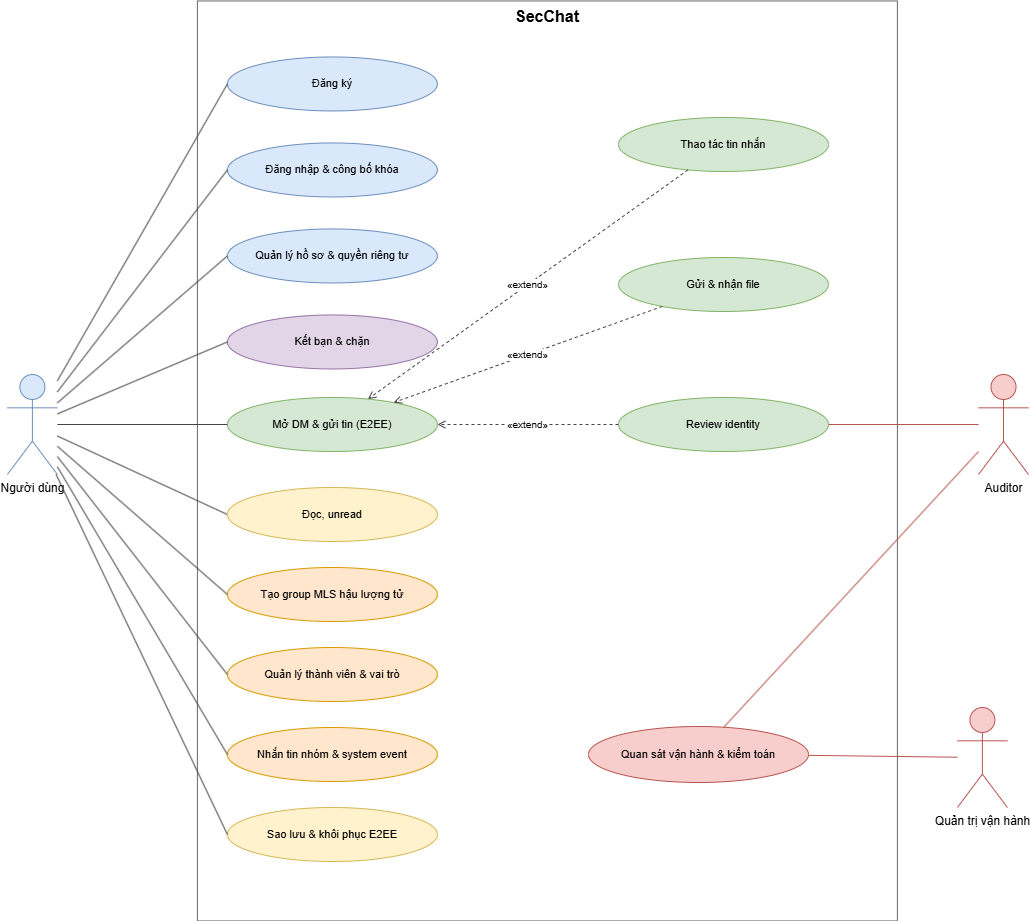
\includegraphics[width=0.95\linewidth]{Figure/UseCaseDiagram.png}
    \caption{Sơ đồ use case tổng quan của SecChat}
    \label{fig:usecase-diagram}
\end{figure}

Các tác nhân tham gia hệ thống gồm:

\begin{itemize}
    \item \textbf{Người dùng:} tác nhân chính của hệ thống. Người dùng thực hiện đăng ký, đăng nhập, kết bạn và chặn, nhắn tin trực tiếp và nhắn tin nhóm được mã hóa đầu cuối, thao tác trên tin nhắn, gửi file, kiểm tra danh tính, quản lý hồ sơ, quyền riêng tư và sao lưu hoặc khôi phục dữ liệu E2EE.
    \item \textbf{Auditor:} dịch vụ minh bạch khóa định danh, hoạt động độc lập với chat server. Auditor đọc log định danh, dựng cây Merkle, ký checkpoint và cấp inclusion proof để client kiểm tra khóa định danh của người khác trước khi tin tưởng.
    \item \textbf{Quản trị vận hành:} người triển khai và giám sát hệ thống qua Docker. Tác nhân này kiểm tra health, readiness, metrics và log qua control plane cùng server GUI, nhưng không có khả năng đọc nội dung tin nhắn của người dùng.
\end{itemize}



\subsection{Đặc tả chức năng}\label{subsec:usecase-spec}

Phần này tóm tắt toàn bộ use case mức hệ thống ở bảng~\ref{tab:usecase-summary}, sau đó đặc tả chi tiết cho bốn use case cốt lõi và phức tạp nhất: đăng nhập và công bố khóa (UC02), mở DM và gửi tin (UC05), quản lý thành viên group MLS (UC10) và sao lưu, khôi phục E2EE (UC13). Các use case còn lại dùng chung cơ chế client gửi lệnh, server kiểm quyền rồi trả event.

\begin{table}[H]
    \centering
    \small
    \begin{tabularx}{\linewidth}{|c|p{0.24\linewidth}|p{0.17\linewidth}|X|}
        \hline
        \textbf{Mã} & \textbf{Use case} & \textbf{Tác nhân} & \textbf{Tóm tắt} \\
        \hline
        UC01 & Đăng ký & Người dùng & Tạo tài khoản, khởi tạo state E2EE và công bố khóa lần đầu. \\ \hline
        UC02 (*) & Đăng nhập và công bố khóa & Người dùng, Auditor & Xác thực, mở local state, công bố PQXDH bundle và MLS KeyPackage. \\ \hline
        UC03 & Quản lý hồ sơ và quyền riêng tư & Người dùng & Cập nhật hồ sơ, avatar, đổi mật khẩu, quyền riêng tư và cache. \\ \hline
        UC04 & Kết bạn và chặn & Người dùng & Tìm, mời, chấp nhận/từ chối kết bạn; chặn/bỏ chặn. \\ \hline
        UC05 (*) & Mở DM và gửi tin & Người dùng, Auditor & Bắt tay PQXDH, gửi \texttt{S3PQI} rồi \texttt{S3DR}; server chỉ lưu ciphertext. \\ \hline
        UC06 & Thao tác tin nhắn & Người dùng & Trả lời, chỉnh sửa, xóa, ghim, thả cảm xúc, chuyển tiếp. \\ \hline
        UC07 & Gửi và nhận file & Người dùng & Mã hóa và gửi tệp đính kèm trong lớp E2EE. \\ \hline
        UC08 & Review identity & Người dùng, Auditor & So sánh safety number qua kênh ngoài, đánh dấu đã xác minh. \\ \hline
        UC09 & Tạo group MLS hậu lượng tử & Người dùng, Server & Tạo group X-Wing, claim KeyPackage; server validate public state. \\ \hline
        UC10 (*) & Quản lý thành viên và vai trò & Admin group & \texttt{prepare}/\texttt{apply}: thêm/xóa/đổi role; server validate \texttt{PublicGroup}. \\ \hline
        UC11 & Nhắn tin nhóm và system event & Thành viên group & Gửi \texttt{S3MLS}; thay đổi membership hiển thị như system event. \\ \hline
        UC12 & Đọc, unread & Người dùng & \texttt{mark\_read} theo message id. \\ \hline
        UC13 (*) & Sao lưu và khôi phục E2EE & Người dùng & Export/restore state mã hóa passphrase; không rollback identity. \\ \hline
        UC14 & Quan sát vận hành và kiểm toán & Quản trị vận hành, Auditor & Kiểm tra health/metrics/log; auditor cấp Merkle proof. \\ \hline
    \end{tabularx}
    \caption{Tổng hợp các use case mức hệ thống ((*): có đặc tả chi tiết bên dưới)}
    \label{tab:usecase-summary}
\end{table}

\subsubsection{UC02 - Đăng nhập và công bố khóa}

\begin{longtable}{|p{0.22\linewidth}|p{0.71\linewidth}|}
\caption{Đặc tả Use Case: Đăng nhập và công bố khóa (UC02)}\label{tab:uc02}\\
\hline
\textbf{Tên Use Case} & Đăng nhập và công bố khóa \\ \hline
\textbf{Tác nhân} & Người dùng (chính), Auditor (phụ) \\ \hline
\textbf{Tiền điều kiện} &
\begin{itemize}
  \item Đã có tài khoản.
  \item Máy hiện tại có local state E2EE, hoặc có backup/identity secret nếu là máy mới.
\end{itemize} \\ \hline
\textbf{Luồng sự kiện chính} &
\begin{enumerate}
  \item Người dùng nhập email và mật khẩu.
  \item Client băm mật khẩu (PBKDF2, salt là email) và gửi gói \texttt{auth}.
  \item Server rate-limit theo (login, IP), xác minh PBKDF2 và đặt trạng thái online.
  \item Client dẫn xuất master key và mở local state đã mã hóa.
  \item Client công bố PQXDH bundle mới cho máy hiện tại và MLS KeyPackage X-Wing.
  \item Server flush notification offline; client tải inbox, danh sách bạn và hội thoại.
\end{enumerate} \\ \hline
\textbf{Luồng sự kiện phát sinh} &
\begin{itemize}
  \item Sai mật khẩu hoặc vượt số lần cho phép: bị khóa tạm thời theo rate limit và báo lỗi.
  \item Máy mới thiếu identity secret: client yêu cầu restore backup hoặc rotate có chủ đích; không tự rotate âm thầm.
\end{itemize} \\ \hline
\textbf{Hậu điều kiện} &
\begin{itemize}
  \item Người dùng online; bundle của máy hiện tại đã được công bố; sẵn sàng gửi và nhận tin.
\end{itemize} \\ \hline
\end{longtable}

\begin{figure}[H]
\centering
\IfFileExists{Figure/ActivityUC02.png}{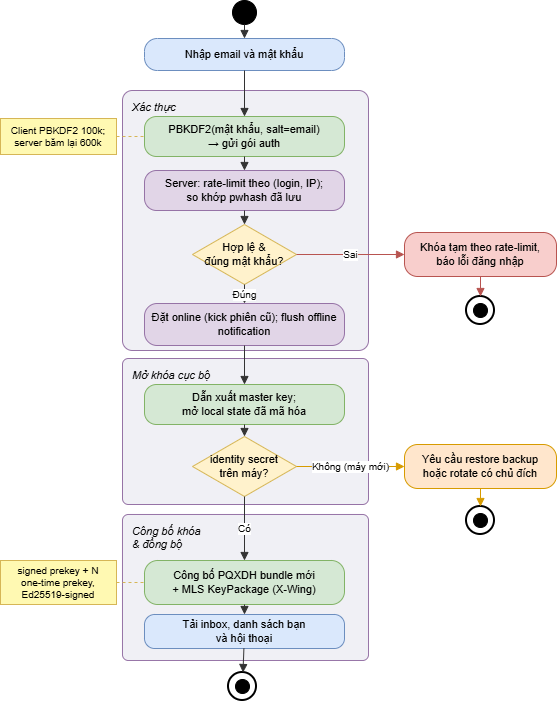
\includegraphics[width=0.72\linewidth]{Figure/ActivityUC02.png}}{\fbox{\parbox[c][3.2cm][c]{0.58\linewidth}{\centering\itshape Sơ đồ hoạt động UC02\\(xuất PNG từ \texttt{diagrams/ActivityUC02.drawio})}}}
\caption{Sơ đồ hoạt động: Đăng nhập và công bố khóa (UC02)}
\label{fig:act-uc02}
\end{figure}

\subsubsection{UC05 - Mở DM và gửi tin}

\begin{longtable}{|p{0.22\linewidth}|p{0.71\linewidth}|}
\caption{Đặc tả Use Case: Mở DM và gửi tin (UC05)}\label{tab:uc05}\\
\hline
\textbf{Tên Use Case} & Mở DM và gửi tin \\ \hline
\textbf{Tác nhân} & Người dùng (chính), Auditor (phụ) \\ \hline
\textbf{Tiền điều kiện} &
\begin{itemize}
  \item Hai bên là bạn hoặc được phép DM; peer đã công bố bundle.
\end{itemize} \\ \hline
\textbf{Luồng sự kiện chính} &
\begin{enumerate}
  \item Client gọi \texttt{start\_dm}; server kiểm tra quyền và chặn tự-DM.
  \item Client gọi \texttt{get\_pqxdh\_bundle}; server trả bundle của peer kèm one-time prekey cùng generation và \texttt{identity\_version}.
  \item Client hỏi auditor lấy Merkle proof cho \texttt{identity\_version} và kiểm tra tính hợp lệ.
  \item Client verify chữ ký prekey, sinh X25519 ephemeral, encapsulate vào ML-KEM của peer, trộn các DH secret và KEM secret bằng HKDF để tạo root secret và khởi tạo Double Ratchet.
  \item Client mã hóa tin đầu tiên và gửi với prefix \texttt{S3PQI}; các tin sau dùng \texttt{S3DR}.
  \item Server lưu ciphertext và chuyển tiếp cho peer; peer giải mã và tiến ratchet.
\end{enumerate} \\ \hline
\textbf{Luồng sự kiện phát sinh} &
\begin{itemize}
  \item Peer thiếu bundle: client báo lỗi rõ và không gửi plaintext.
  \item Bị chặn: server từ chối; bubble đang gửi chuyển sang trạng thái thất bại.
  \item Audit mismatch: hiển thị cảnh báo nhưng vẫn cho gửi (cảnh báo, không chặn).
\end{itemize} \\ \hline
\textbf{Hậu điều kiện} &
\begin{itemize}
  \item Tin được lưu dưới dạng ciphertext; trạng thái ratchet tiến lên.
\end{itemize} \\ \hline
\end{longtable}

\begin{figure}[H]
\centering
\IfFileExists{Figure/ActivityUC05.png}{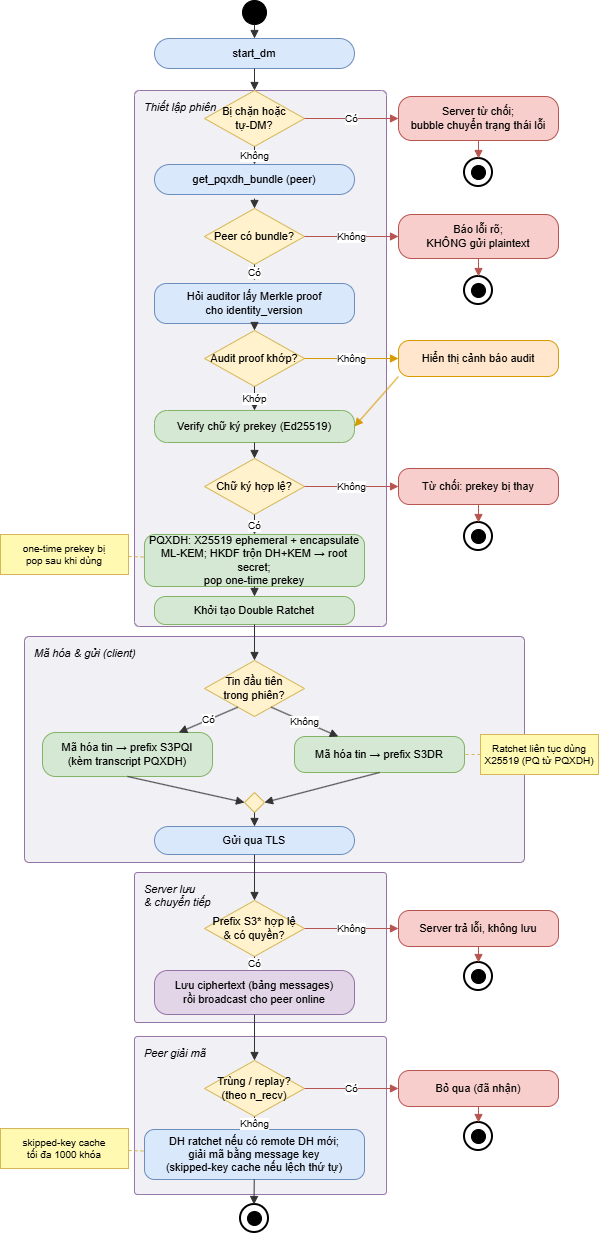
\includegraphics[width=0.72\linewidth]{Figure/ActivityUC05.png}}{\fbox{\parbox[c][3.2cm][c]{0.58\linewidth}{\centering\itshape Sơ đồ hoạt động UC05\\(xuất PNG từ \texttt{diagrams/ActivityUC05.drawio})}}}
\caption{Sơ đồ hoạt động: Mở DM và gửi tin (UC05)}
\label{fig:act-uc05}
\end{figure}

\subsubsection{UC10 - Quản lý thành viên và vai trò}

\begin{longtable}{|p{0.22\linewidth}|p{0.71\linewidth}|}
\caption{Đặc tả Use Case: Quản lý thành viên và vai trò (UC10)}\label{tab:uc10}\\
\hline
\textbf{Tên Use Case} & Quản lý thành viên và vai trò \\ \hline
\textbf{Tác nhân} & Admin group (chính), Server, OpenMLS bridge \\ \hline
\textbf{Tiền điều kiện} &
\begin{itemize}
  \item Là admin (thêm/xóa/đổi role/đổi info) hoặc thành viên (rời nhóm).
\end{itemize} \\ \hline
\textbf{Luồng sự kiện chính} &
\begin{enumerate}
  \item Admin chọn thao tác: thêm/xóa thành viên, đổi role, đổi thông tin nhóm hoặc rời nhóm.
  \item \texttt{prepare\_group\_change}: server kiểm tra policy (quyền admin, friend/block, KeyPackage còn dùng) và tạo operation id.
  \item Client tạo Commit, Welcome và GroupInfo qua OpenMLS.
  \item \texttt{apply\_group\_change}: server validate \texttt{PublicGroup}, đối chiếu member set với pending operation và epoch nối tiếp rồi mutate membership và ghi system event.
\end{enumerate} \\ \hline
\textbf{Luồng sự kiện phát sinh} &
\begin{itemize}
  \item Không phải admin hoặc xóa một admin khác: bị từ chối.
  \item Validation thất bại: handshake không được lưu, membership giữ nguyên.
\end{itemize} \\ \hline
\textbf{Hậu điều kiện} &
\begin{itemize}
  \item Membership và role được cập nhật; system event ghi vào timeline; thành viên bị xóa không nhận epoch mới.
\end{itemize} \\ \hline
\end{longtable}

\begin{figure}[H]
\centering
\IfFileExists{Figure/ActivityUC10.png}{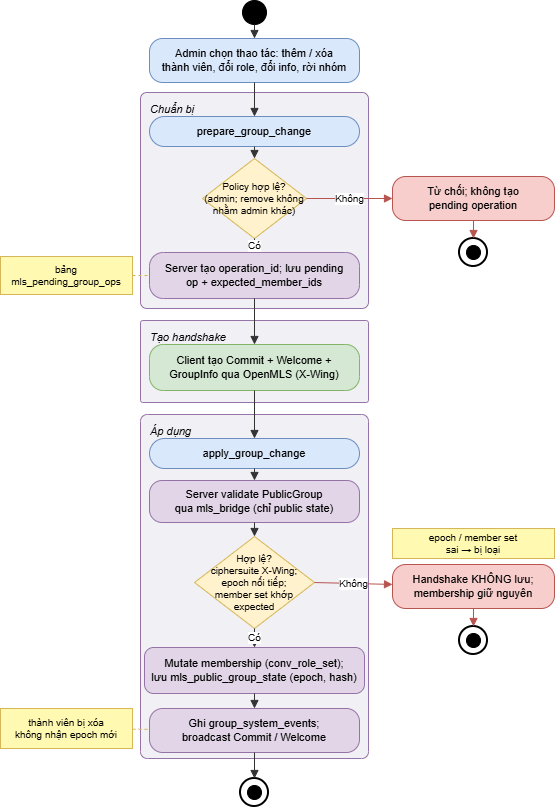
\includegraphics[width=0.72\linewidth]{Figure/ActivityUC10.png}}{\fbox{\parbox[c][3.2cm][c]{0.58\linewidth}{\centering\itshape Sơ đồ hoạt động UC10\\(xuất PNG từ \texttt{diagrams/ActivityUC10.drawio})}}}
\caption{Sơ đồ hoạt động: Quản lý thành viên và vai trò (UC10)}
\label{fig:act-uc10}
\end{figure}

\subsubsection{UC13 - Sao lưu và khôi phục E2EE}

\begin{longtable}{|p{0.22\linewidth}|p{0.71\linewidth}|}
\caption{Đặc tả Use Case: Sao lưu và khôi phục E2EE (UC13)}\label{tab:uc13}\\
\hline
\textbf{Tên Use Case} & Sao lưu và khôi phục E2EE \\ \hline
\textbf{Tác nhân} & Người dùng (chính) \\ \hline
\textbf{Tiền điều kiện} &
\begin{itemize}
  \item Đã đăng nhập (khi sao lưu); có file backup và passphrase (khi khôi phục).
\end{itemize} \\ \hline
\textbf{Luồng sự kiện chính} &
\begin{enumerate}
  \item Người dùng chọn export và chọn có kèm plaintext cache hay không.
  \item Client đóng gói local state (identity, prekey, ratchet, group) và cache tùy chọn, mã hóa bằng PBKDF2(passphrase) cùng AES-GCM với manifest làm AAD.
  \item Khi khôi phục, người dùng mở file, nhập passphrase và client giải mã.
  \item Client re-wrap state bằng master key hiện tại, merge cache theo message id và công bố lại bundle nếu khôi phục được identity secret.
\end{enumerate} \\ \hline
\textbf{Luồng sự kiện phát sinh} &
\begin{itemize}
  \item Sai passphrase: báo lỗi không thể giải mã.
  \item Backup dùng passphrase yếu: bị từ chối.
  \item Khôi phục sau khi đã rotate identity: không rollback identity, chỉ merge cache đọc được.
\end{itemize} \\ \hline
\textbf{Hậu điều kiện} &
\begin{itemize}
  \item Lịch sử đọc được khôi phục cục bộ; server không nhận plaintext.
\end{itemize} \\ \hline
\end{longtable}

\begin{figure}[H]
\centering
\IfFileExists{Figure/ActivityUC13.png}{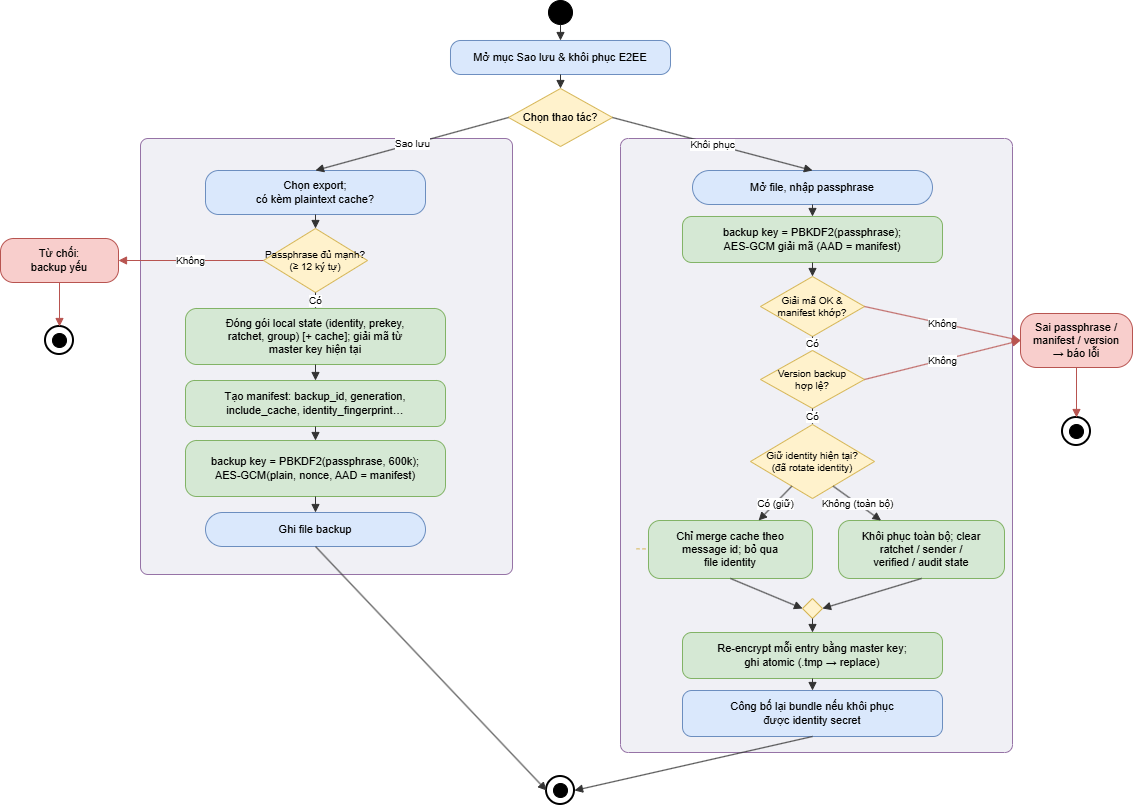
\includegraphics[width=0.98\linewidth]{Figure/ActivityUC13.png}}{\fbox{\parbox[c][3.2cm][c]{0.58\linewidth}{\centering\itshape Sơ đồ hoạt động UC13\\(xuất PNG từ \texttt{diagrams/ActivityUC13.drawio})}}}
\caption{Sơ đồ hoạt động: Sao lưu và khôi phục E2EE (UC13)}
\label{fig:act-uc13}
\end{figure}

\section{Thiết kế hệ thống}

\subsection{Thiết kế cơ sở dữ liệu}

Database của SecChat gồm 20 bảng, không lưu plaintext message, nhưng vẫn lưu metadata cần thiết để hệ thống vận hành. Trường body của bảng \texttt{messages} chỉ chứa ciphertext theo định dạng prefix của giao thức (trình bày ở mục~\ref{subsec:body-format}). Các bảng \texttt{conversation\_members}, \texttt{mls\_group\_state} và \texttt{group\_system\_events} là các điểm quan trọng để bảo đảm group state và timeline ổn định. Các sơ đồ ERD trong mục này là mô hình dữ liệu chính ở mức thiết kế logic. 

\begin{figure}[H]
    \centering
    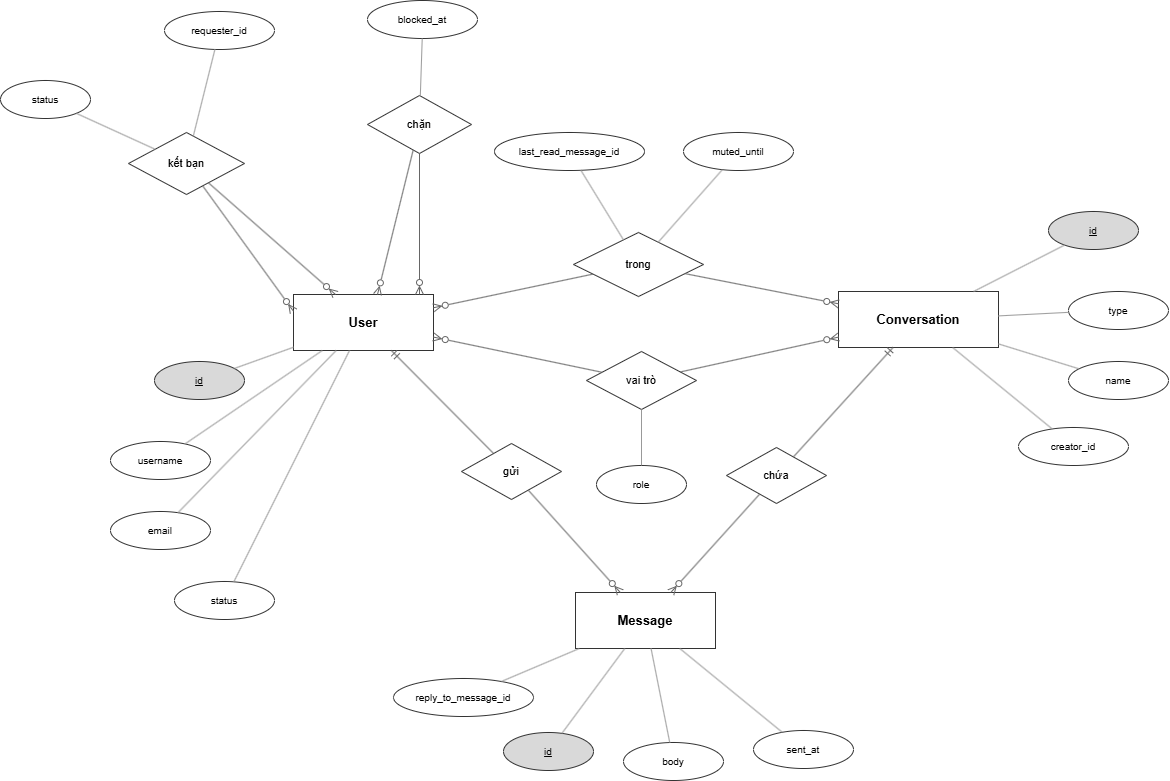
\includegraphics[width=0.96\linewidth]{Figure/ERD_Core.png}
    \caption{ERD phân hệ lõi: người dùng, hội thoại và tin nhắn}
    \label{fig:erd-core}
\end{figure}

\begin{figure}[H]
    \centering
    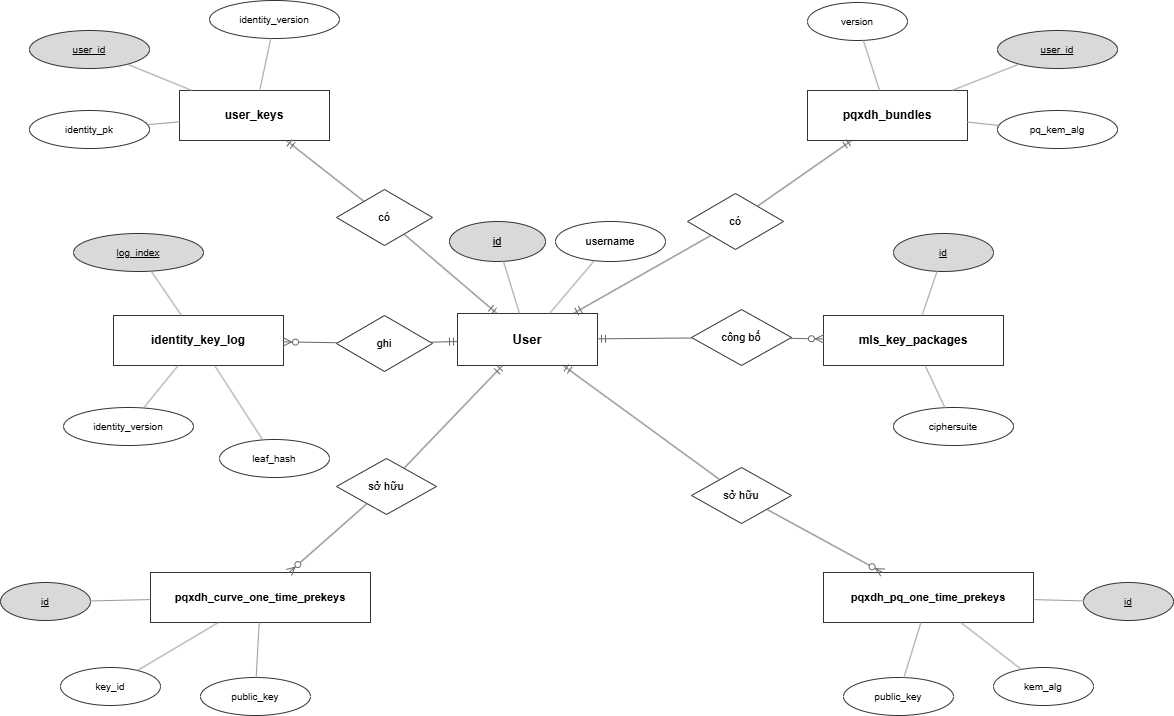
\includegraphics[width=0.96\linewidth]{Figure/ERD_Keys.png}
    \caption{ERD phân hệ khóa và định danh (PQXDH, MLS KeyPackage, identity log)}
    \label{fig:erd-keys}
\end{figure}

\begin{figure}[H]
    \centering
    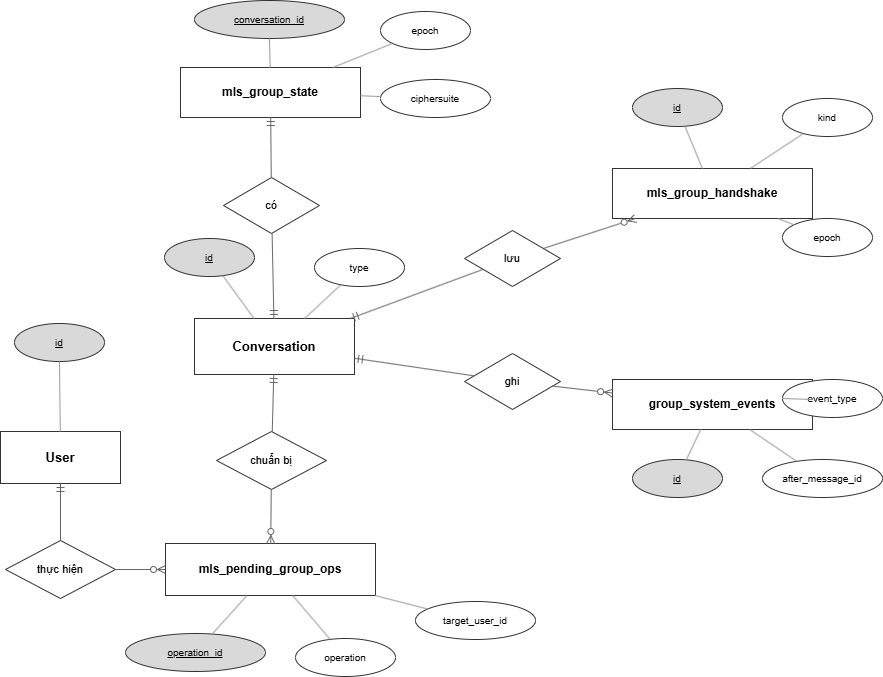
\includegraphics[width=0.92\linewidth]{Figure/ERD_GroupMLS.png}
    \caption{ERD phân hệ nhóm MLS (group state, handshake, system event, pending op)}
    \label{fig:erd-groupmls}
\end{figure}

\begin{figure}[H]
    \centering
    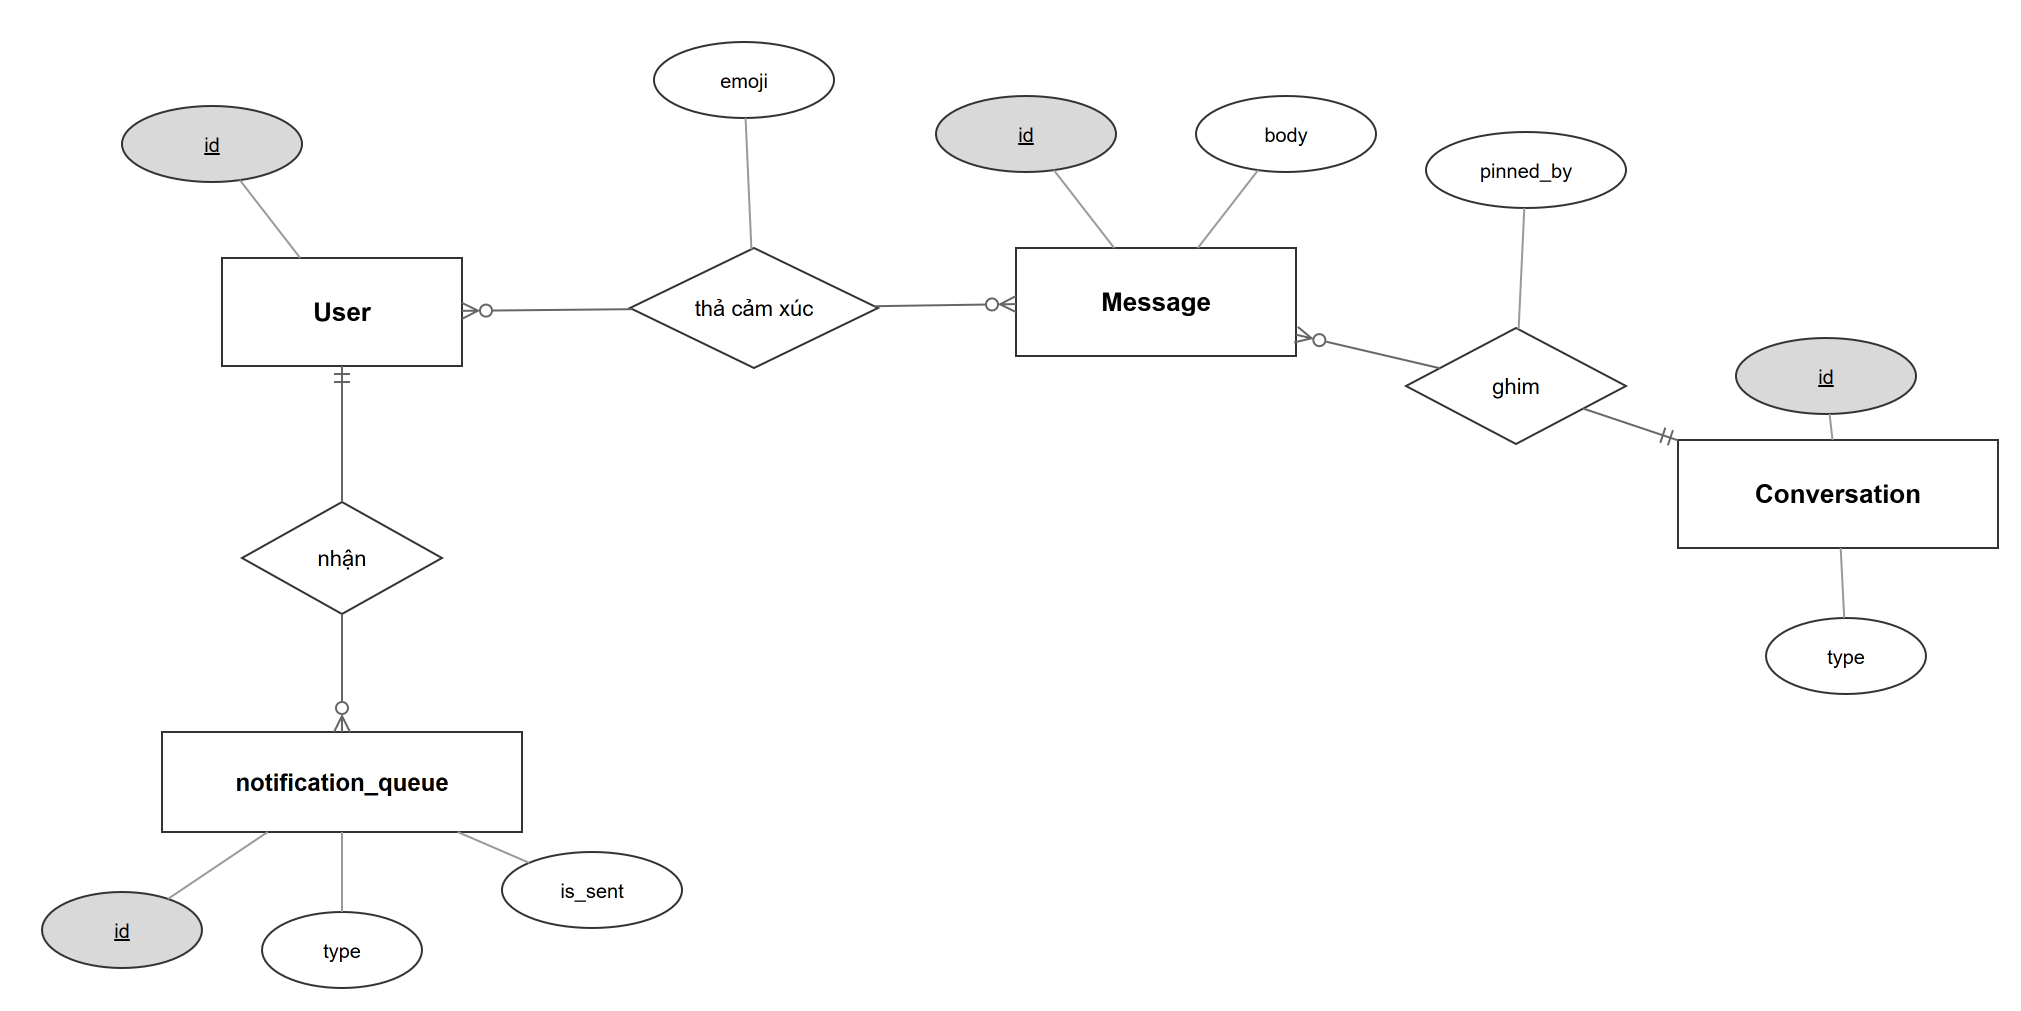
\includegraphics[width=0.96\linewidth]{Figure/ERD_Messaging.png}
    \caption{ERD phân hệ tiện ích tin nhắn và thông báo (reaction, pin, notification)}
    \label{fig:erd-messaging}
\end{figure}

\subsection{Mô tả thực thể}

Bảng mô tả thực thể dưới đây trình bày các thuộc tính chính của từng bảng dữ liệu. Các trường kỹ thuật lặp lại như mốc tạo/cập nhật, cờ trạng thái phụ hoặc dữ liệu phụ trợ chỉ được nêu khi ảnh hưởng trực tiếp đến luồng nghiệp vụ, E2EE, MLS hoặc quan sát vận hành.

{\footnotesize
\begin{longtable}{|p{0.23\linewidth}|p{0.25\linewidth}|p{0.16\linewidth}|p{0.24\linewidth}|}
\caption{Mô tả các thực thể dữ liệu chính}\label{tab:entity-detail}\\
\hline
\textbf{Thực thể} & \textbf{Tên thuộc tính} & \textbf{Kiểu dữ liệu} & \textbf{Mô tả} \\ \hline
\endfirsthead
\hline
\textbf{Thực thể} & \textbf{Tên thuộc tính} & \textbf{Kiểu dữ liệu} & \textbf{Mô tả} \\ \hline
\endhead
\texttt{users} & \texttt{id} & INT, PK & Khóa chính tự tăng. \\ \cline{2-4}
 & \texttt{username} & VARCHAR(64), UNIQUE & Tên đăng nhập. \\ \cline{2-4}
 & \texttt{email} & VARCHAR(200) & Email đăng nhập. \\ \cline{2-4}
 & \texttt{password\_hash} & VARCHAR(200) & Hash mật khẩu (PBKDF2 salt server), không lưu plaintext. \\ \cline{2-4}
 & \texttt{display\_name} & VARCHAR(100) & Tên hiển thị. \\ \cline{2-4}
 & \texttt{avatar} & MEDIUMBLOB & Ảnh đại diện (kèm \texttt{avatar\_mime}). \\ \cline{2-4}
 & \texttt{status} & ENUM (online /offline /away) & Trạng thái hiện diện. \\ \cline{2-4}
 & \texttt{privacy\_online}, \texttt{privacy\_last\_seen} & ENUM (everyone /friends /nobody) & Quyền riêng tư hiện diện. \\ \hline
\texttt{friendships} & \texttt{id} & BIGINT, PK & Khóa chính. \\ \cline{2-4}
 & \texttt{user\_id}, \texttt{friend\_id} & INT, FK & Cặp người dùng trong quan hệ. \\ \cline{2-4}
 & \texttt{requester\_id} & INT, FK & Người gửi lời mời. \\ \cline{2-4}
 & \texttt{status} & ENUM (pending /accepted /blocked) & Trạng thái quan hệ. \\ \hline
\texttt{user\_blocks} & \texttt{blocker\_id} & INT, PK, FK & Người chặn. \\ \cline{2-4}
 & \texttt{blocked\_id} & INT, PK, FK & Người bị chặn. \\ \cline{2-4}
 & \texttt{blocked\_at} & DATETIME & Thời điểm chặn. \\ \hline
\texttt{conversations} & \texttt{id} & BIGINT, PK & Khóa chính. \\ \cline{2-4}
 & \texttt{type} & ENUM (direct /group) & Loại hội thoại. \\ \cline{2-4}
 & \texttt{name} & VARCHAR(100) & Tên nhóm. \\ \cline{2-4}
 & \texttt{creator\_id} & INT, FK & Người tạo nhóm. \\ \cline{2-4}
 & \texttt{description} & TEXT & Mô tả nhóm (kèm \texttt{avatar}). \\ \cline{2-4}
 & \texttt{disappear\_after\_secs} & INT & Thời gian tin tự hủy (kèm \texttt{disappear\_enabled\_at}). \\ \cline{2-4}
 & \texttt{is\_disbanded} & TINYINT(1) & Cờ nhóm đã giải tán. \\ \hline
\texttt{conversation\_members} & \texttt{id} & BIGINT, PK & Khóa chính. \\ \cline{2-4}
 & \texttt{conversation\_id} & BIGINT, FK & Hội thoại. \\ \cline{2-4}
 & \texttt{user\_id} & INT, FK & Thành viên. \\ \cline{2-4}
 & \texttt{last\_read\_message\_id} & BIGINT & Con trỏ đã đọc. \\ \cline{2-4}
 & \texttt{force\_unread} & TINYINT & Đánh dấu chưa đọc thủ công. \\ \cline{2-4}
 & \texttt{muted\_until}, \texttt{conv\_pinned\_at} & DATETIME & Tắt thông báo / ghim hội thoại. \\ \hline
\texttt{group\_roles} & \texttt{conversation\_id} & BIGINT, PK, FK & Nhóm. \\ \cline{2-4}
 & \texttt{user\_id} & INT, PK, FK & Thành viên. \\ \cline{2-4}
 & \texttt{role} & ENUM (admin /member) & Vai trò trong nhóm. \\ \hline
\texttt{messages} & \texttt{id} & BIGINT, PK & Khóa chính. \\ \cline{2-4}
 & \texttt{conversation\_id} & BIGINT, FK & Hội thoại. \\ \cline{2-4}
 & \texttt{sender\_id} & INT, FK & Người gửi. \\ \cline{2-4}
 & \texttt{body} & LONGTEXT & Ciphertext, prefix \texttt{S3PQI}/\texttt{S3DR}/\texttt{S3MLS} (tệp đính kèm là marker \texttt{FILE:} bên trong plaintext đã giải mã). \\ \cline{2-4}
 & \texttt{reply\_to\_message\_id} & BIGINT & Tin được trả lời. \\ \cline{2-4}
 & \texttt{edit\_target\_message\_id} & BIGINT & Tin gốc của event chỉnh sửa. \\ \cline{2-4}
 & \texttt{deleted\_at} & DATETIME(3) & Mốc soft-delete. \\ \hline
\texttt{message\_reactions} & \texttt{id} & BIGINT, PK & Khóa chính. \\ \cline{2-4}
 & \texttt{message\_id} & BIGINT, FK & Tin được thả cảm xúc. \\ \cline{2-4}
 & \texttt{user\_id} & INT, FK & Người thả. \\ \cline{2-4}
 & \texttt{emoji} & VARCHAR(16) & Biểu tượng cảm xúc. \\ \hline
\texttt{pinned\_messages} & \texttt{conversation\_id} & BIGINT, PK, FK & Hội thoại. \\ \cline{2-4}
 & \texttt{message\_id} & BIGINT, PK, FK & Tin được ghim. \\ \cline{2-4}
 & \texttt{pinned\_by} & INT, FK & Người ghim. \\ \hline
\texttt{user\_keys} & \texttt{user\_id} & INT, PK, FK & Chủ sở hữu khóa. \\ \cline{2-4}
 & \texttt{identity\_pk} & TEXT & Ed25519 identity public key. \\ \cline{2-4}
 & \texttt{identity\_sig} & TEXT & Chữ ký tự xác thực identity. \\ \cline{2-4}
 & \texttt{identity\_sk\_enc} & TEXT & Identity secret đã mã hóa bằng master key. \\ \cline{2-4}
 & \texttt{identity\_version} & INT & Phiên bản identity. \\ \hline
\texttt{pqxdh\_bundles} & \texttt{user\_id} & INT, PK, FK & Chủ bundle. \\ \cline{2-4}
 & \texttt{curve\_spk}, \texttt{curve\_spk\_sig} & TEXT & Signed X25519 prekey và chữ ký. \\ \cline{2-4}
 & \texttt{pq\_kem\_alg} & VARCHAR(32) & Tên thuật toán KEM đang dùng (ví dụ \texttt{ML-KEM-1024}). \\ \cline{2-4}
 & \texttt{pq\_spk}, \texttt{pq\_spk\_sig} & TEXT & Signed PQ KEM prekey và chữ ký. \\ \cline{2-4}
 & \texttt{version} & INT & Phiên bản bundle. \\ \hline
\makecell[tl]{\texttt{pqxdh\_curve\_}\\\texttt{one\_time\_prekeys}} & \texttt{id} & BIGINT, PK & Khóa chính. \\ \cline{2-4}
 & \texttt{user\_id} & INT, FK & Chủ prekey. \\ \cline{2-4}
 & \texttt{key\_id} & INT & Định danh prekey. \\ \cline{2-4}
 & \texttt{public\_key}, \texttt{signature} & TEXT & One-time X25519 prekey và chữ ký. \\ \hline
\makecell[tl]{\texttt{pqxdh\_pq\_}\\\texttt{one\_time\_prekeys}} & \texttt{id} & BIGINT, PK & Khóa chính. \\ \cline{2-4}
 & \texttt{user\_id} & INT, FK & Chủ prekey. \\ \cline{2-4}
 & \texttt{kem\_alg} & VARCHAR(32) & Thuật toán KEM. \\ \cline{2-4}
 & \texttt{public\_key}, \texttt{signature} & TEXT & One-time PQ KEM prekey và chữ ký. \\ \hline
\texttt{identity\_key\_log} & \texttt{log\_index} & BIGINT, PK & Chỉ số append-only. \\ \cline{2-4}
 & \texttt{user\_id} & INT, FK & Chủ identity. \\ \cline{2-4}
 & \texttt{identity\_version} & INT & Phiên bản identity. \\ \cline{2-4}
 & \texttt{identity\_pk} & TEXT & Identity key tại version đó. \\ \cline{2-4}
 & \texttt{event\_type} & ENUM (initial /rotation) & Loại sự kiện. \\ \cline{2-4}
 & \texttt{leaf\_hash} & CHAR(64) & Hash lá Merkle. \\ \hline
\texttt{mls\_key\_packages} & \texttt{id} & BIGINT, PK & Khóa chính. \\ \cline{2-4}
 & \texttt{user\_id} & INT, FK & Chủ KeyPackage. \\ \cline{2-4}
 & \texttt{ciphersuite} & VARCHAR(128) & Ciphersuite X-Wing. \\ \cline{2-4}
 & \texttt{key\_package\_b64} & LONGTEXT & KeyPackage MLS (base64). \\ \cline{2-4}
 & \texttt{secchat\_signature} & TEXT & Chữ ký SecChat trên KeyPackage. \\ \cline{2-4}
 & \texttt{claimed\_at}, \texttt{claimed\_by} & DATETIME(3), INT & Trạng thái đã claim (single-use). \\ \hline
\texttt{mls\_group\_state} & \texttt{conversation\_id} & BIGINT, PK, FK & Nhóm. \\ \cline{2-4}
 & \texttt{group\_id\_b64} & VARCHAR(256) & Group id MLS. \\ \cline{2-4}
 & \texttt{epoch} & BIGINT & Epoch hiện hành. \\ \cline{2-4}
 & \texttt{ciphersuite} & VARCHAR(128) & Ciphersuite X-Wing. \\ \cline{2-4}
 & \texttt{public\_state\_b64} & LONGTEXT & Public group state đã validate. \\ \cline{2-4}
 & \texttt{public\_state\_hash}, \texttt{validated\_at} & VARCHAR(128), DATETIME(3) & Hash và mốc validate. \\ \hline
\texttt{mls\_pending\_group\_ops} & \texttt{operation\_id} & VARCHAR(64), PK & Định danh operation. \\ \cline{2-4}
 & \texttt{conversation\_id} & BIGINT, FK & Nhóm. \\ \cline{2-4}
 & \texttt{actor\_id} & INT, FK & Người thực hiện. \\ \cline{2-4}
 & \texttt{operation} & VARCHAR(32) & Loại thao tác (add/remove/...). \\ \cline{2-4}
 & \texttt{target\_user\_id} & INT & Đối tượng tác động. \\ \cline{2-4}
 & \texttt{status} & ENUM (prepared /applied /rejected) & Trạng thái; \texttt{expires\_at} giới hạn thời gian. \\ \hline
\texttt{mls\_group\_handshake} & \texttt{id} & BIGINT, PK & Khóa chính. \\ \cline{2-4}
 & \texttt{conversation\_id} & BIGINT, FK & Nhóm. \\ \cline{2-4}
 & \texttt{kind} & ENUM (welcome /commit /group\_info /control) & Loại artifact MLS. \\ \cline{2-4}
 & \texttt{epoch} & BIGINT & Epoch của artifact. \\ \cline{2-4}
 & \texttt{operation\_id} & VARCHAR(64) & Operation liên quan. \\ \cline{2-4}
 & \texttt{mls\_message\_b64} & LONGTEXT & Bytes MLS (base64) để client replay. \\ \hline
\texttt{group\_system\_events} & \texttt{id} & BIGINT, PK & Khóa chính. \\ \cline{2-4}
 & \texttt{conversation\_id} & BIGINT, FK & Nhóm. \\ \cline{2-4}
 & \texttt{event\_type} & VARCHAR(32) & Loại sự kiện (add/remove/role/...). \\ \cline{2-4}
 & \texttt{target\_user\_id}, \texttt{role} & INT, VARCHAR(16) & Đối tượng và vai trò. \\ \cline{2-4}
 & \texttt{operation\_id} & VARCHAR(64) & Khử trùng lặp với realtime. \\ \cline{2-4}
 & \texttt{after\_message\_id} & BIGINT & Vị trí trong timeline. \\ \hline
\texttt{notification\_queue} & \texttt{id} & BIGINT, PK & Khóa chính. \\ \cline{2-4}
 & \texttt{user\_id} & INT, FK & Người nhận. \\ \cline{2-4}
 & \texttt{type} & VARCHAR(64) & Loại notification. \\ \cline{2-4}
 & \texttt{payload} & TEXT & Nội dung sự kiện. \\ \cline{2-4}
 & \texttt{is\_sent} & TINYINT & Đã flush hay chưa. \\ \hline
\end{longtable}
}

\subsection{Thiết kế cấu trúc đối tượng}

Sơ đồ class diagram trong mục này mô tả các lớp và module chính của hệ thống ở mức thiết kế. Mỗi lớp chỉ nêu các thuộc tính và phương thức tiêu biểu thể hiện trách nhiệm của thành phần đó.

\begin{figure}[H]
    \centering
    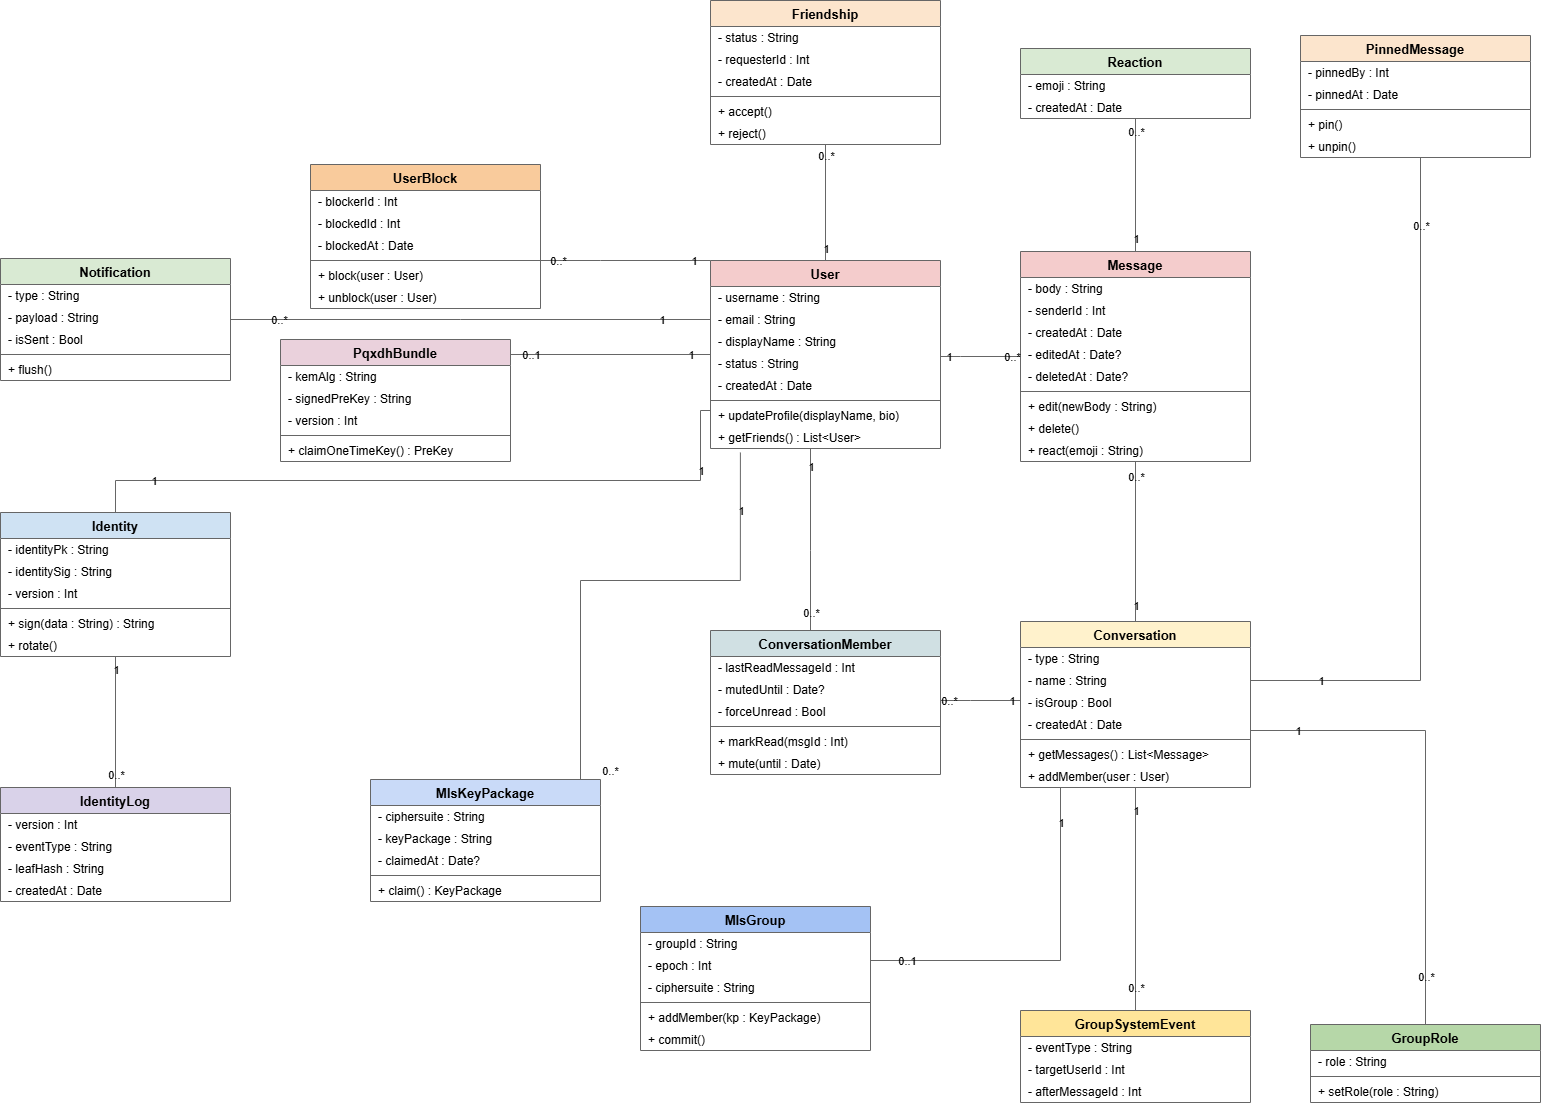
\includegraphics[width=0.98\linewidth]{Figure/ClassDiagramCore.png}
    \caption{Sơ đồ class diagram các lớp chính của hệ thống}
    \label{fig:class-detail}
\end{figure}

\textbf{1. Class: User}

{\small
\begin{longtable}{|p{0.25\linewidth}|p{0.14\linewidth}|p{0.28\linewidth}|p{0.21\linewidth}|}
\hline
\textbf{Tên} & \textbf{Loại} & \textbf{Kiểu dữ liệu / Tham số} & \textbf{Mô tả} \\ \hline
\endhead
\texttt{username} & Thuộc tính & String & Tên đăng nhập (duy nhất). \\ \hline
\texttt{email} & Thuộc tính & String & Email đăng nhập. \\ \hline
\texttt{displayName} & Thuộc tính & String & Tên hiển thị. \\ \hline
\texttt{status} & Thuộc tính & String & Trạng thái hiện diện (online/offline). \\ \hline
\texttt{createdAt} & Thuộc tính & Date & Ngày tạo tài khoản. \\ \hline
\texttt{updateProfile} & Phương thức & displayName, bio & Cập nhật hồ sơ. \\ \hline
\texttt{getFriends} & Phương thức & $\rightarrow$ List\textless User\textgreater  & Lấy danh sách bạn bè. \\ \hline
\end{longtable}
}

\textbf{2. Class: Friendship}

{\small
\begin{longtable}{|p{0.25\linewidth}|p{0.14\linewidth}|p{0.28\linewidth}|p{0.21\linewidth}|}
\hline
\textbf{Tên} & \textbf{Loại} & \textbf{Kiểu dữ liệu / Tham số} & \textbf{Mô tả} \\ \hline
\endhead
\texttt{status} & Thuộc tính & String & Trạng thái (pending/accepted/ blocked). \\ \hline
\texttt{requesterId} & Thuộc tính & Int & Người gửi lời mời. \\ \hline
\texttt{createdAt} & Thuộc tính & Date & Thời điểm tạo. \\ \hline
\texttt{accept} & Phương thức & void & Chấp nhận lời mời. \\ \hline
\texttt{reject} & Phương thức & void & Từ chối lời mời. \\ \hline
\end{longtable}
}

\textbf{3. Class: UserBlock}

{\small
\begin{longtable}{|p{0.25\linewidth}|p{0.14\linewidth}|p{0.28\linewidth}|p{0.21\linewidth}|}
\hline
\textbf{Tên} & \textbf{Loại} & \textbf{Kiểu dữ liệu / Tham số} & \textbf{Mô tả} \\ \hline
\endhead
\texttt{blockerId} & Thuộc tính & Int & Người chặn. \\ \hline
\texttt{blockedId} & Thuộc tính & Int & Người bị chặn. \\ \hline
\texttt{blockedAt} & Thuộc tính & Date & Thời điểm chặn. \\ \hline
\texttt{block} & Phương thức & user: User & Chặn một người dùng. \\ \hline
\texttt{unblock} & Phương thức & user: User & Bỏ chặn. \\ \hline
\end{longtable}
}

\textbf{4. Class: Notification}

{\small
\begin{longtable}{|p{0.25\linewidth}|p{0.14\linewidth}|p{0.28\linewidth}|p{0.21\linewidth}|}
\hline
\textbf{Tên} & \textbf{Loại} & \textbf{Kiểu dữ liệu / Tham số} & \textbf{Mô tả} \\ \hline
\endhead
\texttt{type} & Thuộc tính & String & Loại thông báo. \\ \hline
\texttt{payload} & Thuộc tính & String & Nội dung sự kiện. \\ \hline
\texttt{isSent} & Thuộc tính & Bool & Đã đẩy tới client hay chưa. \\ \hline
\texttt{flush} & Phương thức & void & Đẩy thông báo còn tồn khi user online. \\ \hline
\end{longtable}
}

\textbf{5. Class: IdentityLog}

{\small
\begin{longtable}{|p{0.25\linewidth}|p{0.14\linewidth}|p{0.28\linewidth}|p{0.21\linewidth}|}
\hline
\textbf{Tên} & \textbf{Loại} & \textbf{Kiểu dữ liệu / Tham số} & \textbf{Mô tả} \\ \hline
\endhead
\texttt{version} & Thuộc tính & Int & Phiên bản identity tại sự kiện. \\ \hline
\texttt{eventType} & Thuộc tính & String & Loại sự kiện (initial/rotation). \\ \hline
\texttt{leafHash} & Thuộc tính & String & Hash lá trong cây Merkle minh bạch. \\ \hline
\texttt{createdAt} & Thuộc tính & Date & Thời điểm ghi log. \\ \hline
\end{longtable}
}

\textbf{6. Class: Identity}

{\small
\begin{longtable}{|p{0.25\linewidth}|p{0.14\linewidth}|p{0.28\linewidth}|p{0.21\linewidth}|}
\hline
\textbf{Tên} & \textbf{Loại} & \textbf{Kiểu dữ liệu / Tham số} & \textbf{Mô tả} \\ \hline
\endhead
\texttt{identityPk} & Thuộc tính & String & Khóa định danh công khai Ed25519. \\ \hline
\texttt{identitySig} & Thuộc tính & String & Chữ ký tự xác thực. \\ \hline
\texttt{version} & Thuộc tính & Int & Phiên bản identity. \\ \hline
\texttt{sign} & Phương thức & data: String $\rightarrow$ String & Ký prekey/dữ liệu. \\ \hline
\texttt{rotate} & Phương thức & void & Xoay sang identity key mới. \\ \hline
\end{longtable}
}

\textbf{7. Class: PqxdhBundle}

{\small
\begin{longtable}{|p{0.25\linewidth}|p{0.14\linewidth}|p{0.28\linewidth}|p{0.21\linewidth}|}
\hline
\textbf{Tên} & \textbf{Loại} & \textbf{Kiểu dữ liệu / Tham số} & \textbf{Mô tả} \\ \hline
\endhead
\texttt{kemAlg} & Thuộc tính & String & Thuật toán KEM (ML-KEM-1024). \\ \hline
\texttt{signedPreKey} & Thuộc tính & String & Signed prekey đã ký. \\ \hline
\texttt{version} & Thuộc tính & Int & Phiên bản bundle. \\ \hline
\texttt{claimOneTimeKey} & Phương thức & $\rightarrow$ PreKey & Cấp một one-time prekey. \\ \hline
\end{longtable}
}

\textbf{8. Class: MlsKeyPackage}

{\small
\begin{longtable}{|p{0.25\linewidth}|p{0.14\linewidth}|p{0.28\linewidth}|p{0.21\linewidth}|}
\hline
\textbf{Tên} & \textbf{Loại} & \textbf{Kiểu dữ liệu / Tham số} & \textbf{Mô tả} \\ \hline
\endhead
\texttt{ciphersuite} & Thuộc tính & String & Ciphersuite X-Wing. \\ \hline
\texttt{keyPackage} & Thuộc tính & String & KeyPackage MLS (base64). \\ \hline
\texttt{claimedAt} & Thuộc tính & Date? & Thời điểm bị claim (single-use). \\ \hline
\texttt{claim} & Phương thức & $\rightarrow$ KeyPackage & Lấy KeyPackage để thêm vào nhóm. \\ \hline
\end{longtable}
}

\textbf{9. Class: Conversation}

{\small
\begin{longtable}{|p{0.25\linewidth}|p{0.14\linewidth}|p{0.28\linewidth}|p{0.21\linewidth}|}
\hline
\textbf{Tên} & \textbf{Loại} & \textbf{Kiểu dữ liệu / Tham số} & \textbf{Mô tả} \\ \hline
\endhead
\texttt{type} & Thuộc tính & String & Loại (direct/group). \\ \hline
\texttt{name} & Thuộc tính & String & Tên nhóm. \\ \hline
\texttt{isGroup} & Thuộc tính & Bool & Cờ nhóm/DM. \\ \hline
\texttt{createdAt} & Thuộc tính & Date & Ngày tạo. \\ \hline
\texttt{getMessages} & Phương thức & $\rightarrow$ List\textless Message\textgreater  & Lấy danh sách tin. \\ \hline
\texttt{addMember} & Phương thức & user: User & Thêm thành viên. \\ \hline
\end{longtable}
}

\textbf{10. Class: ConversationMember}

{\small
\begin{longtable}{|p{0.25\linewidth}|p{0.14\linewidth}|p{0.28\linewidth}|p{0.21\linewidth}|}
\hline
\textbf{Tên} & \textbf{Loại} & \textbf{Kiểu dữ liệu / Tham số} & \textbf{Mô tả} \\ \hline
\endhead
\texttt{lastReadMessageId} & Thuộc tính & Int & Con trỏ đã đọc. \\ \hline
\texttt{mutedUntil} & Thuộc tính & Date? & Tắt thông báo đến thời điểm. \\ \hline
\texttt{forceUnread} & Thuộc tính & Bool & Đánh dấu chưa đọc thủ công. \\ \hline
\texttt{markRead} & Phương thức & msgId: Int & Đánh dấu đã đọc tới msgId. \\ \hline
\texttt{mute} & Phương thức & until: Date & Tắt thông báo hội thoại. \\ \hline
\end{longtable}
}

\textbf{11. Class: GroupRole}

{\small
\begin{longtable}{|p{0.25\linewidth}|p{0.14\linewidth}|p{0.28\linewidth}|p{0.21\linewidth}|}
\hline
\textbf{Tên} & \textbf{Loại} & \textbf{Kiểu dữ liệu / Tham số} & \textbf{Mô tả} \\ \hline
\endhead
\texttt{role} & Thuộc tính & String & Vai trò (admin/member). \\ \hline
\texttt{setRole} & Phương thức & role: String & Đặt vai trò thành viên. \\ \hline
\end{longtable}
}

\textbf{12. Class: MlsGroup}

{\small
\begin{longtable}{|p{0.25\linewidth}|p{0.14\linewidth}|p{0.28\linewidth}|p{0.21\linewidth}|}
\hline
\textbf{Tên} & \textbf{Loại} & \textbf{Kiểu dữ liệu / Tham số} & \textbf{Mô tả} \\ \hline
\endhead
\texttt{groupId} & Thuộc tính & String & Định danh group MLS. \\ \hline
\texttt{epoch} & Thuộc tính & Int & Epoch hiện hành. \\ \hline
\texttt{ciphersuite} & Thuộc tính & String & X-Wing (ML-KEM-768 + X25519). \\ \hline
\texttt{addMember} & Phương thức & kp: KeyPackage & Thêm thành viên, sinh Commit/Welcome. \\ \hline
\texttt{commit} & Phương thức & void & Áp thay đổi, tiến epoch. \\ \hline
\end{longtable}
}

\textbf{13. Class: Message}

{\small
\begin{longtable}{|p{0.25\linewidth}|p{0.14\linewidth}|p{0.28\linewidth}|p{0.21\linewidth}|}
\hline
\textbf{Tên} & \textbf{Loại} & \textbf{Kiểu dữ liệu / Tham số} & \textbf{Mô tả} \\ \hline
\endhead
\texttt{body} & Thuộc tính & String & Nội dung đã mã hóa (ciphertext). \\ \hline
\texttt{senderId} & Thuộc tính & Int & Người gửi. \\ \hline
\texttt{createdAt} & Thuộc tính & Date & Thời điểm gửi. \\ \hline
\texttt{editedAt} & Thuộc tính & Date? & Thời điểm sửa (null nếu chưa). \\ \hline
\texttt{deletedAt} & Thuộc tính & Date? & Thời điểm thu hồi (null nếu chưa). \\ \hline
\texttt{edit} & Phương thức & newBody: String & Sửa nội dung. \\ \hline
\texttt{delete} & Phương thức & void & Thu hồi (soft-delete). \\ \hline
\texttt{react} & Phương thức & emoji: String & Thả cảm xúc. \\ \hline
\end{longtable}
}

\textbf{14. Class: Reaction}

{\small
\begin{longtable}{|p{0.25\linewidth}|p{0.14\linewidth}|p{0.28\linewidth}|p{0.21\linewidth}|}
\hline
\textbf{Tên} & \textbf{Loại} & \textbf{Kiểu dữ liệu / Tham số} & \textbf{Mô tả} \\ \hline
\endhead
\texttt{emoji} & Thuộc tính & String & Biểu tượng cảm xúc. \\ \hline
\texttt{createdAt} & Thuộc tính & Date & Thời điểm thả. \\ \hline
\end{longtable}
}

\textbf{15. Class: PinnedMessage}

{\small
\begin{longtable}{|p{0.25\linewidth}|p{0.14\linewidth}|p{0.28\linewidth}|p{0.21\linewidth}|}
\hline
\textbf{Tên} & \textbf{Loại} & \textbf{Kiểu dữ liệu / Tham số} & \textbf{Mô tả} \\ \hline
\endhead
\texttt{pinnedBy} & Thuộc tính & Int & Người ghim. \\ \hline
\texttt{pinnedAt} & Thuộc tính & Date & Thời điểm ghim. \\ \hline
\texttt{pin} & Phương thức & void & Ghim tin. \\ \hline
\texttt{unpin} & Phương thức & void & Bỏ ghim. \\ \hline
\end{longtable}
}

\textbf{16. Class: GroupSystemEvent}

{\small
\begin{longtable}{|p{0.25\linewidth}|p{0.14\linewidth}|p{0.28\linewidth}|p{0.21\linewidth}|}
\hline
\textbf{Tên} & \textbf{Loại} & \textbf{Kiểu dữ liệu / Tham số} & \textbf{Mô tả} \\ \hline
\endhead
\texttt{eventType} & Thuộc tính & String & Loại sự kiện (add/remove/role...). \\ \hline
\texttt{targetUserId} & Thuộc tính & Int & Đối tượng tác động. \\ \hline
\texttt{afterMessageId} & Thuộc tính & Int & Vị trí trong dòng thời gian. \\ \hline
\end{longtable}
}

\subsection{Thiết kế luồng xử lý}

Mục này đặc tả các luồng nghiệp vụ chính dưới dạng sơ đồ tuần tự, mô tả trình tự trao đổi thông điệp giữa client, server, database, auditor và OpenMLS bridge. Các luồng phụ như sao lưu/khôi phục E2EE và kiểm tra identity transparency đã được trình bày dưới dạng sơ đồ luồng ở mục~\ref{sec:security-protocol}.

\textbf{Quy trình đăng nhập và công bố khóa}

Sau khi xác thực thành công, client mở local state đã mã hóa và công bố lại bundle khóa của máy hiện tại để người khác có thể bắt đầu hội thoại ngay cả khi chủ tài khoản offline.

\begin{figure}[H]
    \centering
    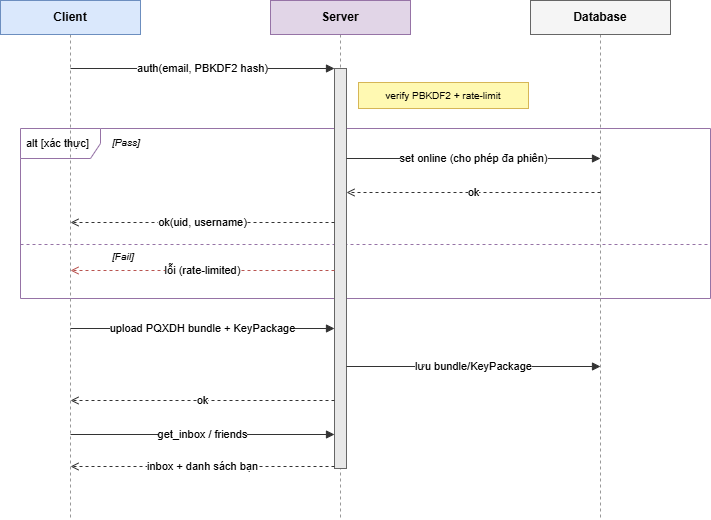
\includegraphics[width=0.85\linewidth]{Figure/SequenceLoginKeyPublish.png}
    \caption{Sơ đồ tuần tự: đăng nhập và công bố khóa}
    \label{fig:seq-login-key-publish}
\end{figure}

\textbf{Quy trình gửi tin nhắn DM E2EE}

Client lấy bundle của peer, kiểm tra proof identity với auditor, thực hiện bắt tay PQXDH để tạo root secret rồi gửi tin đã mã hóa; server chỉ lưu và chuyển tiếp ciphertext.

\begin{figure}[H]
    \centering
    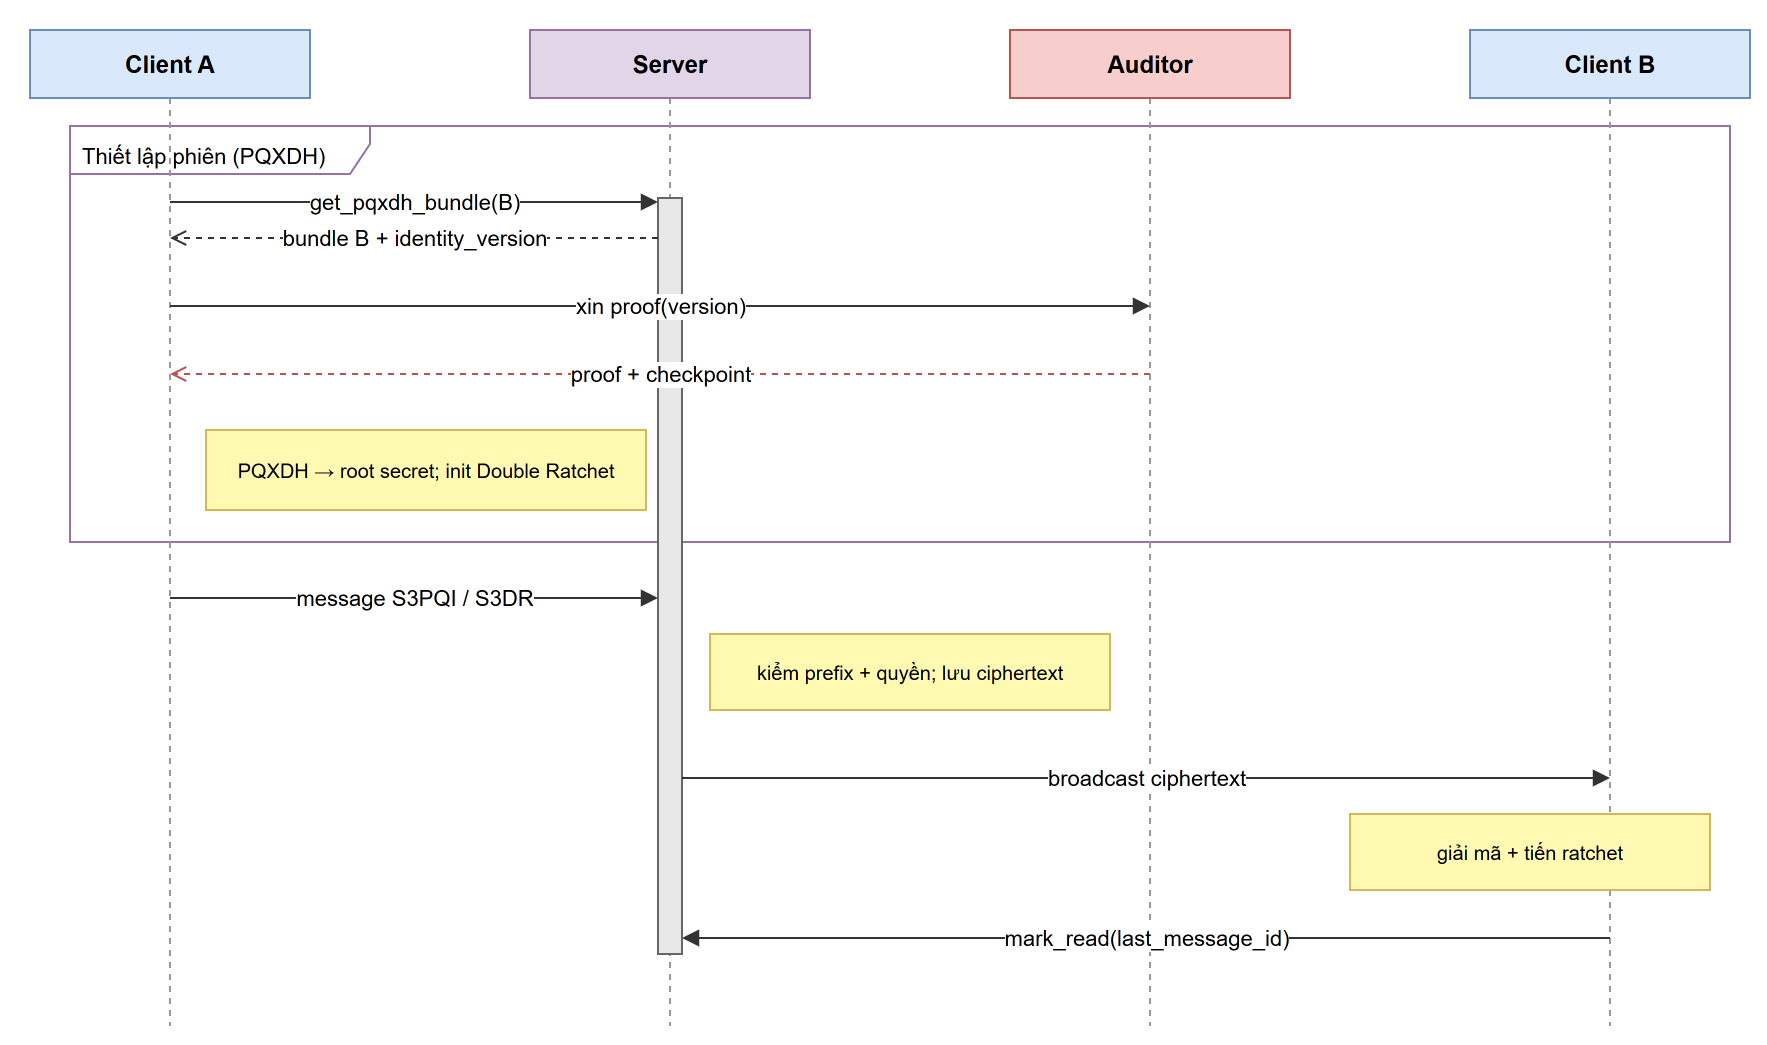
\includegraphics[width=0.9\linewidth]{Figure/SequenceDmE2ee.png}
    \caption{Sơ đồ tuần tự: gửi tin nhắn DM E2EE}
    \label{fig:seq-dm-e2ee}
\end{figure}

\textbf{Quy trình thay đổi thành viên group bằng MLS}

Mọi thay đổi membership đi qua hai bước \texttt{prepare} và \texttt{apply}; server chỉ áp dụng thay đổi sau khi MLS validator chấp nhận public state dựa trên \texttt{PublicGroup}.

\begin{figure}[H]
    \centering
    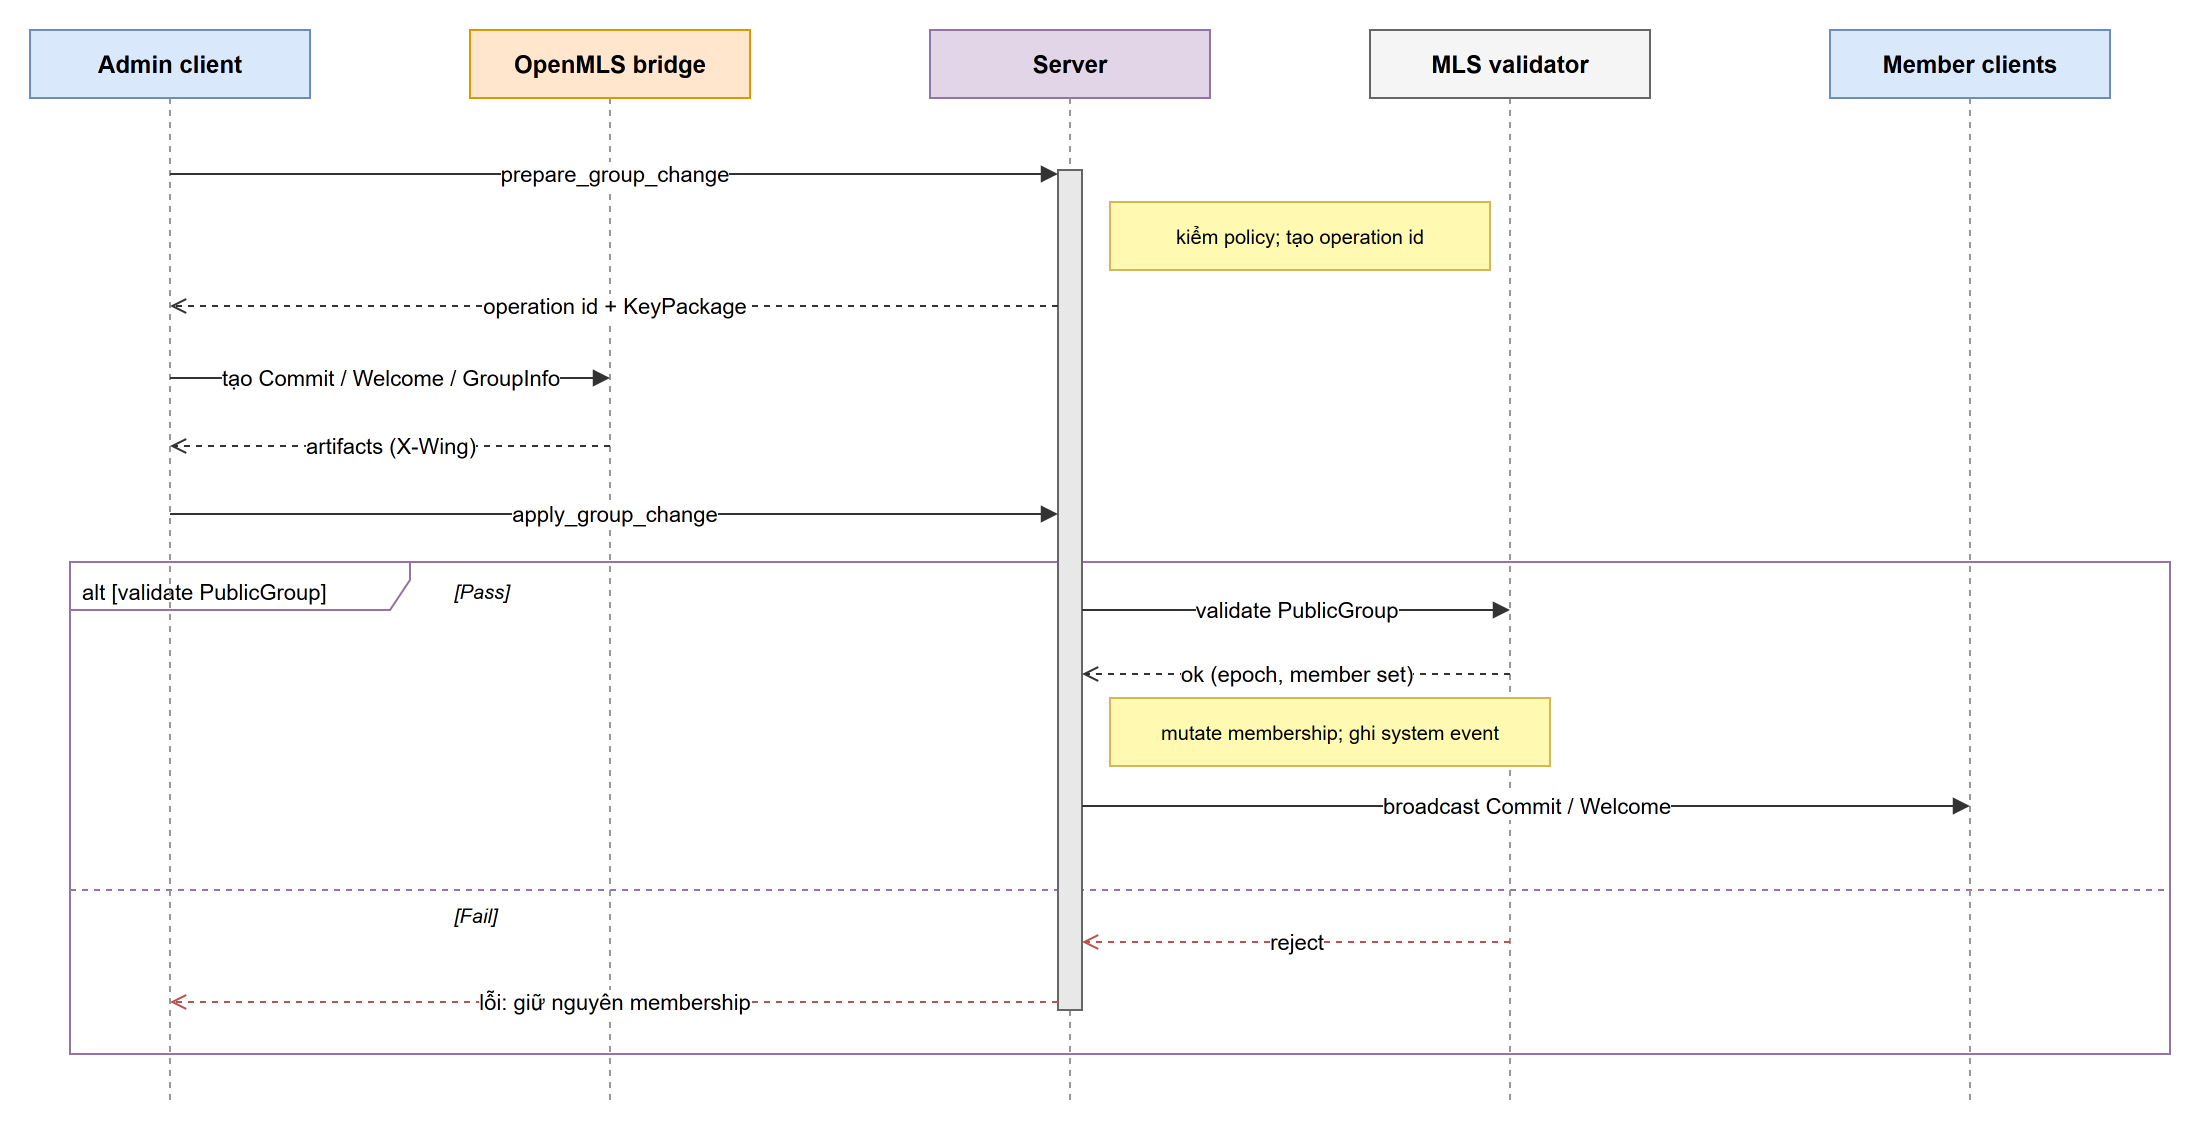
\includegraphics[width=0.95\linewidth]{Figure/SequenceGroupMlsValidation.png}
    \caption{Sơ đồ tuần tự: thay đổi thành viên group bằng MLS}
    \label{fig:seq-group-mls-validation}
\end{figure}

\textbf{Quy trình tải lịch sử, read cursor và system event}

Khi mở hội thoại, client cập nhật read cursor theo message id và tải lịch sử ciphertext cùng các system event để dựng lại timeline đúng thứ tự sau khi đăng nhập lại hoặc reload.

\begin{figure}[H]
    \centering
    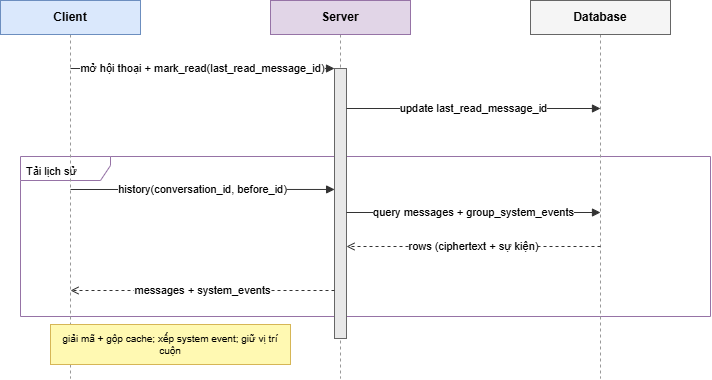
\includegraphics[width=0.85\linewidth]{Figure/SequenceHistoryReadSystemEvents.png}
    \caption{Sơ đồ tuần tự: tải lịch sử, read cursor và system event}
    \label{fig:seq-history-read-events}
\end{figure}

\section{Thiết kế giao thức bảo mật}\label{sec:security-protocol}

Yêu cầu thiết kế quan trọng nhất là server không được đọc nội dung tin nhắn người dùng. Tin nhắn phải được mã hóa ở client trước khi gửi lên server. Server có thể lưu, chuyển tiếp, sắp xếp và trả lịch sử, nhưng trường nội dung trong cơ sở dữ liệu phải là ciphertext có prefix hợp lệ của giao thức.

Với group, hệ thống dùng MLS theo RFC 9420 qua OpenMLS để quản lý epoch, secret tree, Welcome và Commit. Ciphersuite group là X-Wing hybrid, kết hợp ML-KEM-768 với X25519 cho confidentiality và dùng Ed25519 cho authentication; X-Wing hiện là bản nháp Internet-Draft (\texttt{draft-connolly-cfrg-xwing-kem}) mang tính thực nghiệm. Server phải từ chối KeyPackage không đúng ciphersuite, kiểm tra chữ ký SecChat trên KeyPackage, và validate public MLS state trước khi mutate membership.

Khóa bí mật của người dùng không được lưu thô. Client phải mã hóa identity key, prekey, ratchet state, group state và các file trạng thái E2EE bằng master key dẫn xuất từ mật khẩu. Khi người dùng đổi mật khẩu, các file nhạy cảm cục bộ phải được bọc lại bằng master key mới.

Client được tin tưởng để giữ plaintext, master key và trạng thái crypto. Server được tin tưởng để xác thực tài khoản, kiểm tra quyền trong group, validate public MLS state, lưu thứ tự tin nhắn và chuyển tiếp đúng người, nhưng không được tin tưởng để giữ bí mật nội dung tin.

Cơ sở dữ liệu được xem là có thể bị lộ. Vì vậy các secret quan trọng phải được lưu ở dạng mã hóa.


\subsection{Thiết kế mã hóa đầu cuối}

\subsubsection{Các lớp khóa}

SecChat tách khóa theo vai trò thay vì dùng một khóa chung cho toàn bộ hệ thống. Identity key Ed25519 gắn với danh tính bảo mật của tài khoản và dùng để ký prekey. Prekey X25519 và prekey ML-KEM dùng cho bắt tay DM kiểu PQXDH. Sau bắt tay, Double Ratchet state tạo message key riêng cho từng tin DM. Với group, OpenMLS giữ MLS group state, epoch secret và application secret; server chỉ thấy public state cần cho kiểm tra membership.

Cách chia này giúp mỗi khóa có vòng đời rõ ràng. Mật khẩu dùng để mở khóa local state, identity key dùng để nhận diện người dùng, prekey dùng để bắt tay phiên, còn message key dùng cho từng tin nhắn.

\begin{figure}[H]
    \centering
    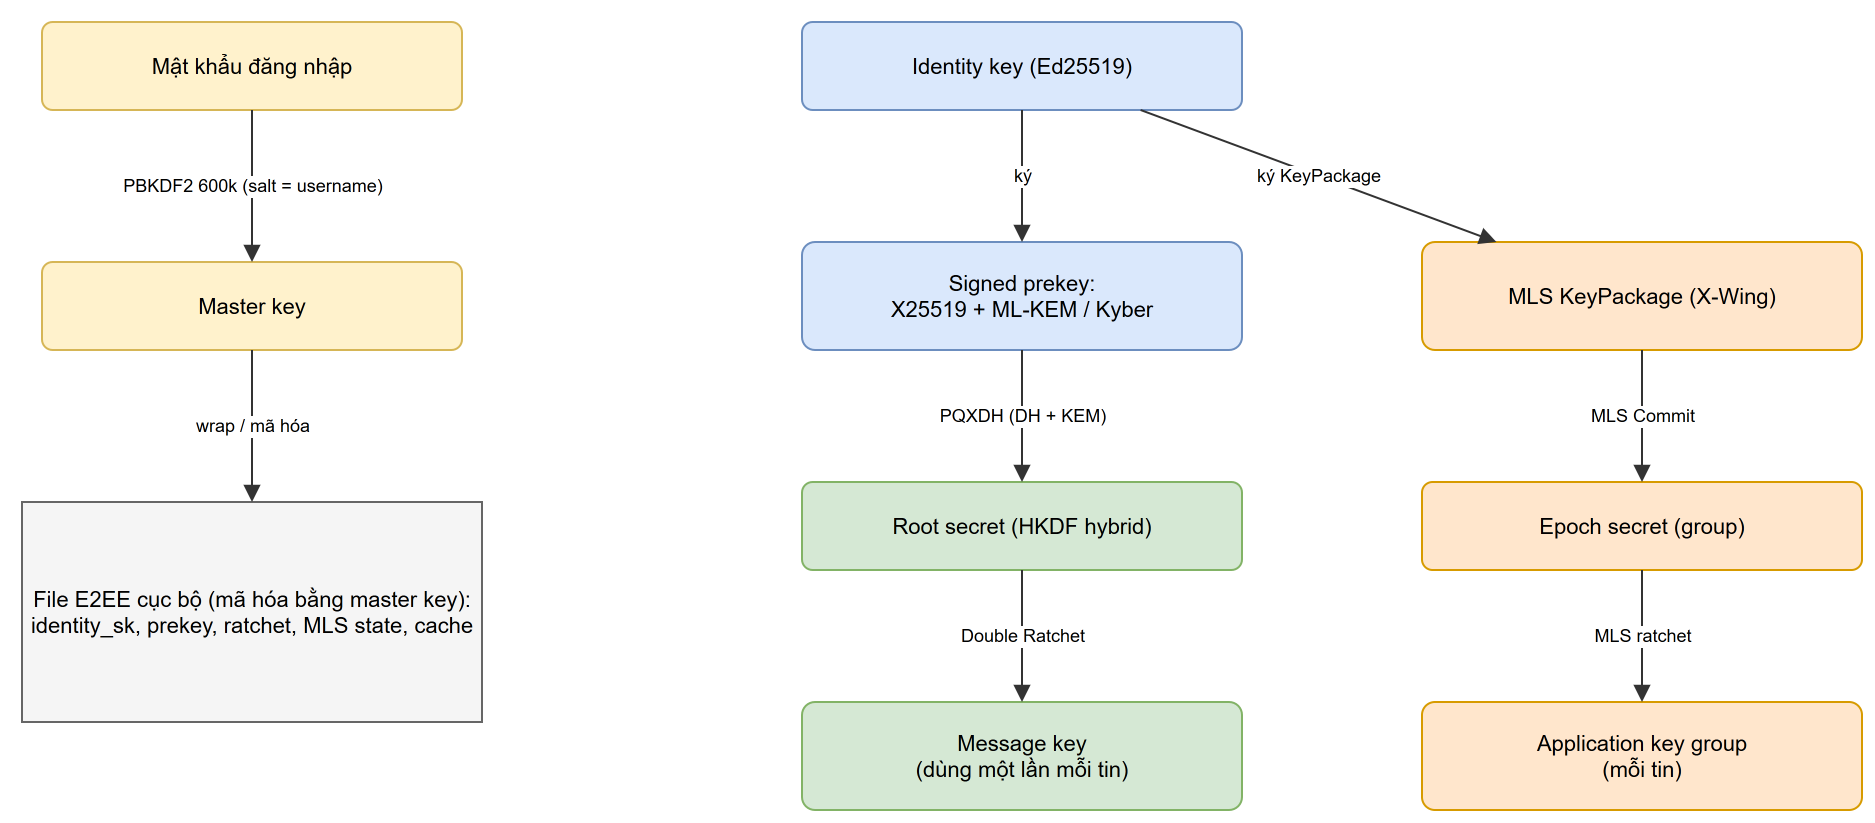
\includegraphics[width=0.9\linewidth]{Figure/KeyLifecycle.png}
    \caption{Vòng đời các khóa chính trong SecChat}
    \label{fig:keylifecycle}
\end{figure}

\subsubsection{Mật khẩu và master key}\label{subsubsec:password}

Ở tầng đăng nhập, client không gửi mật khẩu thô lên server. Client trước hết băm mật khẩu bằng PBKDF2-HMAC-SHA256 với salt là email đăng nhập. Server tiếp tục băm giá trị nhận được bằng PBKDF2 với salt ngẫu nhiên riêng trước khi lưu vào bảng \texttt{users}. Thiết kế này làm cho server không biết mật khẩu gốc.

Ở tầng bảo vệ file E2EE cục bộ, client dẫn xuất master key từ mật khẩu gốc và username thực tế do server trả về sau đăng nhập. Master key này dùng để mã hóa các file như identity secret key, prekey secret, ratchet state, group state, safety verification và plaintext cache. Khi đổi mật khẩu, client bọc lại các file này bằng master key mới để lịch sử và key cũ không bị mất.

\subsubsection{Prekey bundle kiểu PQXDH}

Mỗi client công bố một bundle khóa cho SecChat. Bundle gồm identity public key Ed25519, signed X25519 prekey, signed ML-KEM prekey, cùng các one-time prekey nếu còn. Bắt tay DM ưu tiên ML-KEM-1024 khi thư viện hỗ trợ, nhưng bundle vẫn ghi rõ thuật toán đang dùng để hai phía xử lý đúng. Server lưu bundle trong các bảng như \texttt{pqxdh\_bundles}, \texttt{pqxdh\_curve\_one\_time\_prekeys} và \texttt{pqxdh\_pq\_one\_time\_prekeys}.

Khi cùng một tài khoản đăng nhập trên thiết bị khác, nếu mở được identity secret, client sẽ tạo một PQXDH bundle mới cho thiết bị hiện tại và upload lại trước khi nhận hoặc gửi DM mới. Cách này giữ nguyên safety identity nhưng thay prekey theo máy đang active, tránh tình trạng server trả bundle có public prekey không khớp với secret cục bộ. Nếu server đang có bundle cũ nhưng client hiện tại thiếu private prekey, client vẫn phải publish bundle mới thay vì dựa vào trạng thái cũ.

Khi A muốn bắt đầu DM với B, A gọi \texttt{get\_pqxdh\_bundle}. Server trả bundle của B và chỉ cấp one-time prekey thuộc cùng generation với signed prekey hiện hành. Khi B publish bundle mới, server xóa batch one-time prekey cũ trước khi chèn batch mới; nhờ vậy người gửi không bị nhận signed prekey mới ghép với one-time prekey cũ. Bundle trả về có thêm \texttt{identity\_version}. Trước khi dùng bundle, client hỏi auditor service để lấy Merkle proof cho identity key và version đó. Kết quả audit được lưu vào security state của hội thoại: proof hợp lệ làm tăng độ tin cậy; proof, key, version hoặc checkpoint sai được ghi là \texttt{audit\_mismatch} với mã lỗi cụ thể; lỗi vận hành như auditor không truy cập được hoặc HTTP lỗi được ghi là \texttt{audit\_unavailable}. Client kiểm tra chữ ký prekey bằng identity key của B, sinh X25519 ephemeral, encapsulate vào ML-KEM public key của B, rồi trộn các DH secret và KEM secret bằng HKDF. Secret đầu ra dùng để khởi tạo Double Ratchet.

Identity transparency không thay thế safety number. Nó giúp client biết key đang dùng có nằm trong lịch sử identity đã được auditor ký hay không. Nếu safety number đổi, UI đánh dấu hội thoại là key changed và yêu cầu người dùng mở phần review để xem lịch sử identity trước khi tiếp tục gửi tin một cách bình thường. Nếu proof root không khớp, identity version không có trong log, identity key trong bundle khác log, checkpoint rollback, checkpoint split-view hoặc chữ ký checkpoint sai, UI hiển thị cảnh báo audit kèm nguyên nhân cụ thể. Nếu auditor tạm thời không truy cập được, UI cũng báo rõ đây là lỗi khả dụng của auditor, không đánh đồng với lỗi bằng chứng mật mã. Các cảnh báo này nhắc người dùng rằng chưa nên tin danh tính của đối phương nếu chưa so sánh safety number qua kênh ngoài SecChat. Cần phân biệt rõ hai loại: cảnh báo identity ở đây mang tính tư vấn, nghĩa là hệ thống hiển thị banner và trạng thái cần review nhưng không tự chặn cứng việc gửi tin, quyết định cuối cùng thuộc về người dùng; còn các lỗi crypto thật như chữ ký bundle sai, thiếu prekey cục bộ hoặc không có group Welcome thì làm việc mã hóa không thể tiếp tục.

\begin{figure}[H]
    \centering
    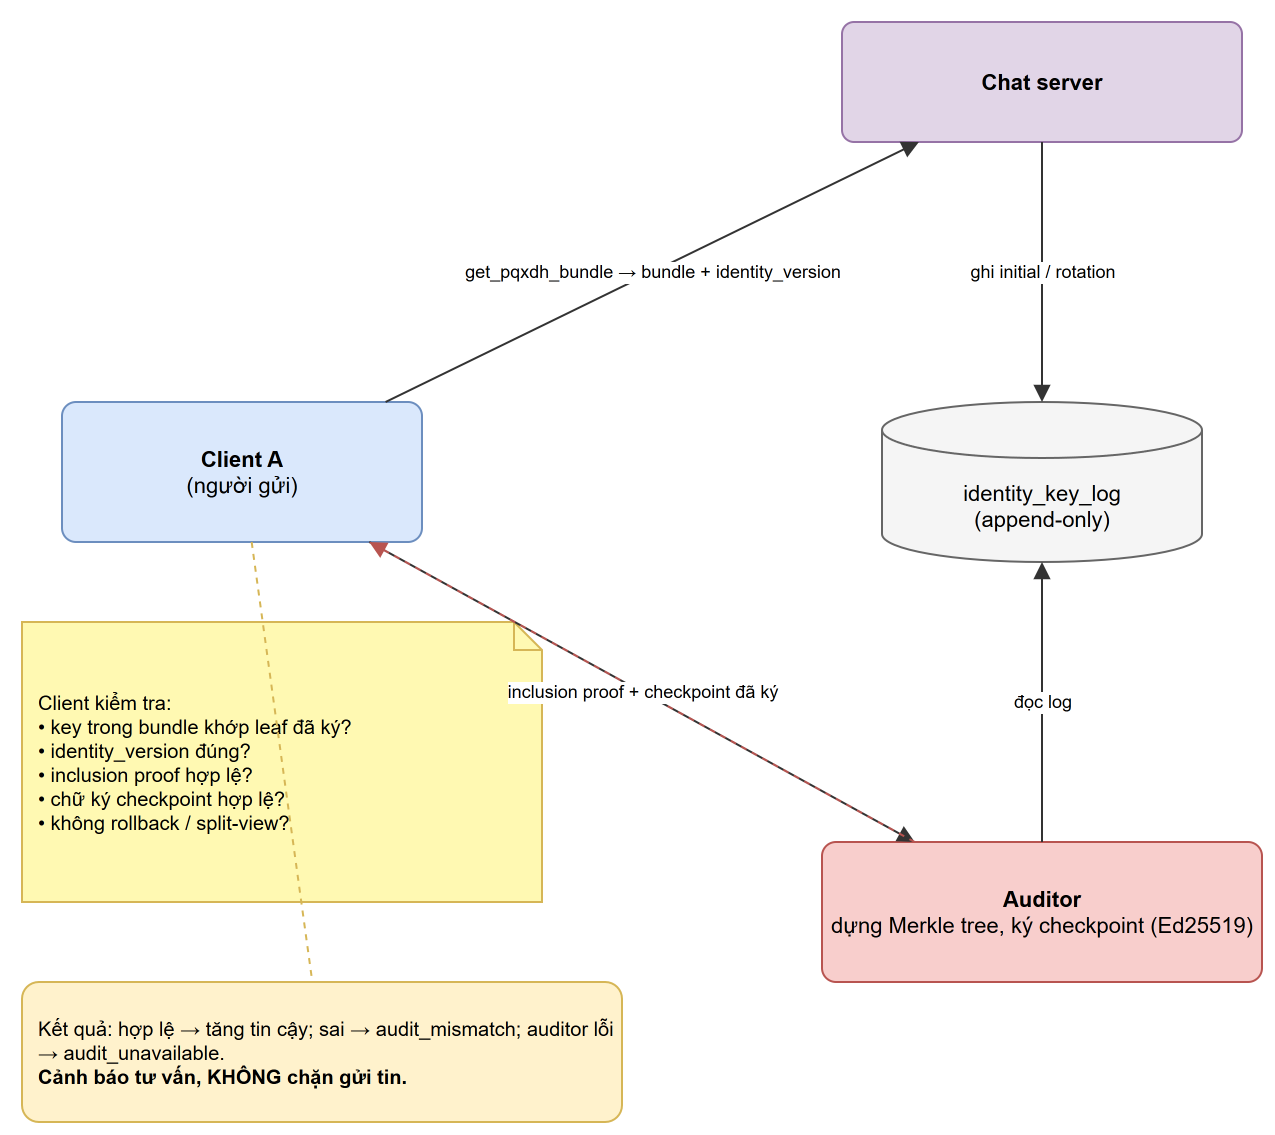
\includegraphics[width=0.9\linewidth]{Figure/IdentityTransparencyFlow.png}
    \caption{Luồng identity transparency giữa client, chat server và auditor}
    \label{fig:identitytransparencyflow}
\end{figure}

Tin nhắn đầu tiên của DM có prefix \texttt{S3PQI:}. Prefix này chứa transcript cần thiết để B tính lại cùng root secret và nhận tin đầu tiên. Sau đó các tin DM bình thường dùng prefix \texttt{S3DR:}. Toàn bộ trình tự lấy bundle, kiểm tra proof, sinh root secret rồi gửi tin đầu tiên được minh họa ở sơ đồ tuần tự~\ref{fig:seq-dm-e2ee}.

Chi tiết mật mã của bước bắt tay được trình bày ở Hình~\ref{fig:seq-pqxdh-kyber}: A trộn ba X25519 DH với shared secret ML-KEM-1024 bằng HKDF để tạo root secret; B decapsulate rồi tính lại đúng root đó. Đây là tính chất hybrid - kẻ tấn công phải phá đồng thời cả X25519 lẫn ML-KEM mới thu được root.

\begin{figure}[H]
    \centering
    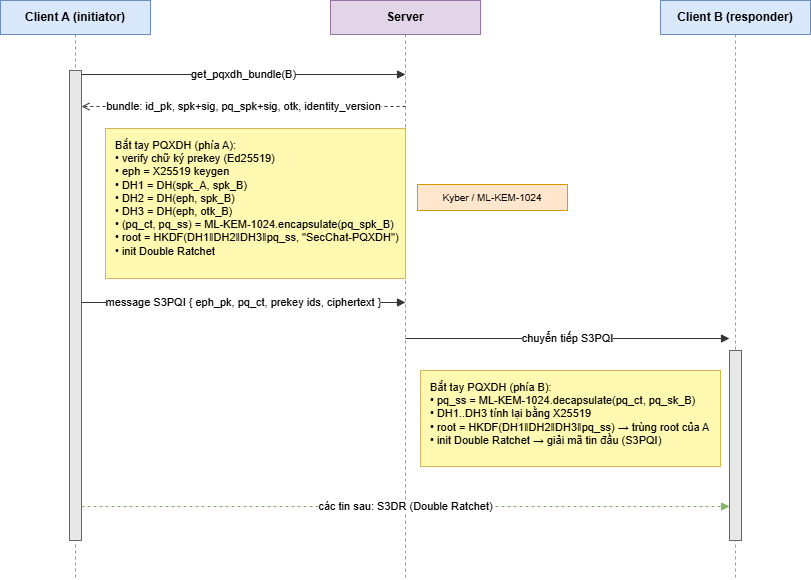
\includegraphics[width=0.92\linewidth]{Figure/SequencePqxdhKyber.png}
    \caption{Sơ đồ tuần tự: bắt tay PQXDH hybrid (X25519 + ML-KEM-1024)}
    \label{fig:seq-pqxdh-kyber}
\end{figure}

\subsubsection{Double Ratchet cho DM}

Sau khi DM được thiết lập, root key ban đầu lấy từ bắt tay PQXDH, rồi từ đó mỗi tin được mã hóa bằng một message key dùng một lần.

Về định dạng truyền, tin đầu tiên của phiên mang prefix \texttt{S3PQI} (gói kèm dữ liệu bắt tay PQXDH), các tin sau mang prefix \texttt{S3DR}. Bộ nhớ skipped-key được giới hạn 1000 khóa để chịu được tin offline và tin lệch thứ tự mà không bị làm cạn bộ nhớ. Toàn bộ trạng thái ratchet được mã hóa bằng master key rồi lưu trên đĩa, nên người dùng đăng xuất rồi đăng nhập lại vẫn tiếp tục đúng phiên mà không mất lịch sử.

\begin{figure}[H]
    \centering
    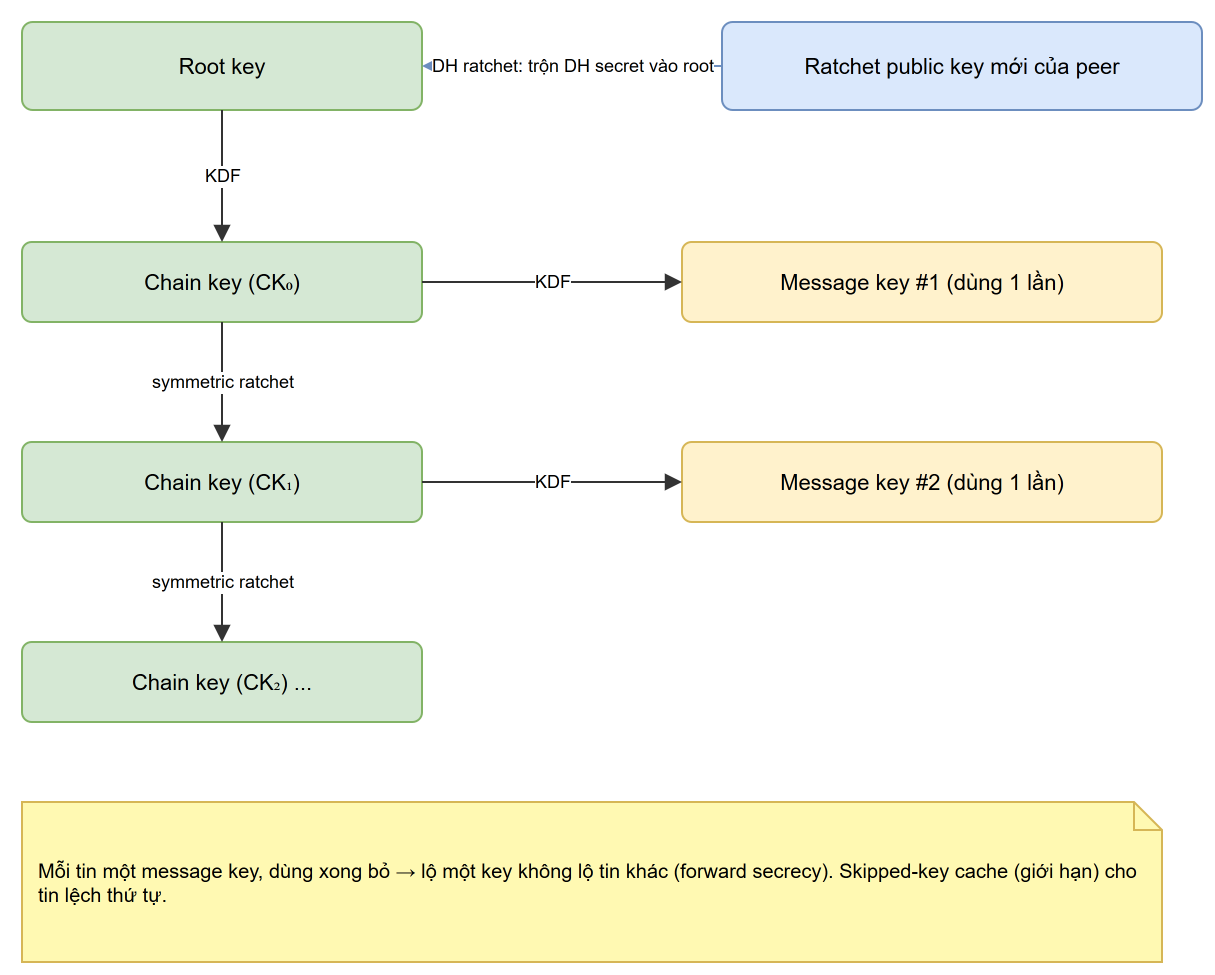
\includegraphics[width=0.9\linewidth]{Figure/DoubleRatchetFlow.png}
    \caption{Luồng Double Ratchet cho tin nhắn DM}
    \label{fig:doubleratchetflow}
\end{figure}


\subsubsection{Group MLS hậu lượng tử hybrid}\label{subsubsec:group-mls}

Nhóm chat không dùng Double Ratchet theo từng cặp mà dùng MLS với một group state chung có cấu trúc cây. SecChat hiện thực điều này bằng OpenMLS, chạy MLS theo RFC 9420 với ciphersuite X-Wing:
\begin{center}
    \small\texttt{MLS\_256\_XWING\_CHACHA20POLY1305\_SHA256\_Ed25519}
\end{center}
X-Wing là KEM hybrid kết hợp ML-KEM-768 và X25519, cung cấp bảo vệ hậu lượng tử cho confidentiality của group còn phần authentication của MLS sử dụng chữ ký Ed25519 cổ điển. Như đã nêu ở Chương 1, X-Wing hiện vẫn là một bản nháp Internet-Draft mang tính thực nghiệm chứ chưa phải chuẩn đã ổn định.

Mỗi thành viên công bố KeyPackage X-Wing sau khi đăng nhập. KeyPackage được ký thêm bằng SecChat identity key để server và client kiểm tra rằng package thuộc đúng tài khoản và đúng identity version. Server từ chối KeyPackage không đúng ciphersuite hoặc sai chữ ký trước khi lưu vào bảng \texttt{mls\_key\_packages}. Nếu client mở local MLS state cũ không còn khớp ciphersuite X-Wing, state đó bị bỏ và client công bố lại KeyPackage mới.

Mỗi thay đổi membership dùng Commit và GroupInfo do OpenMLS sinh. Luồng thay đổi bắt đầu bằng bước prepare: server kiểm tra policy như quyền admin, friend/block và KeyPackage còn chưa dùng. Client sau đó dùng OpenMLS bridge để tạo Commit, Welcome, GroupInfo và ratchet tree cần thiết, rồi gửi lại ở bước apply. Trước khi lưu handshake hoặc cập nhật bảng thành viên, server gọi validator OpenMLS dựa trên \texttt{PublicGroup}. Validator kiểm tra ciphersuite X-Wing, group id của conversation, epoch nối tiếp, credential của actor và member set sau commit có khớp operation đang chờ hay không. Trình tự prepare/apply giữa admin client, OpenMLS bridge, server và MLS validator được minh họa ở sơ đồ tuần tự~\ref{fig:seq-group-mls-validation}.

Public MLS state đã validate được lưu trong \texttt{mls\_group\_state}, gồm ciphersuite, public state base64, public state hash, backend validation và thời điểm validate. Server vẫn không giữ epoch secret, không sinh group secret và không giải mã MLS application bytes. Thành viên mới nhận Welcome dành riêng cho KeyPackage của mình và không mặc nhiên đọc được lịch sử trước khi tham gia. Thành viên bị xóa xử lý Commit remove thì group local inactive và không đọc được tin sau epoch mới.

Toàn bộ vòng đời khóa MLS - công bố KeyPackage X-Wing, tạo Commit/Welcome/GroupInfo, server validate \texttt{PublicGroup}, thành viên \texttt{join\_from\_welcome} và mã hóa application message (\texttt{S3MLS}) - được mô tả ở Hình~\ref{fig:seq-mls-group}.

\begin{figure}[H]
    \centering
    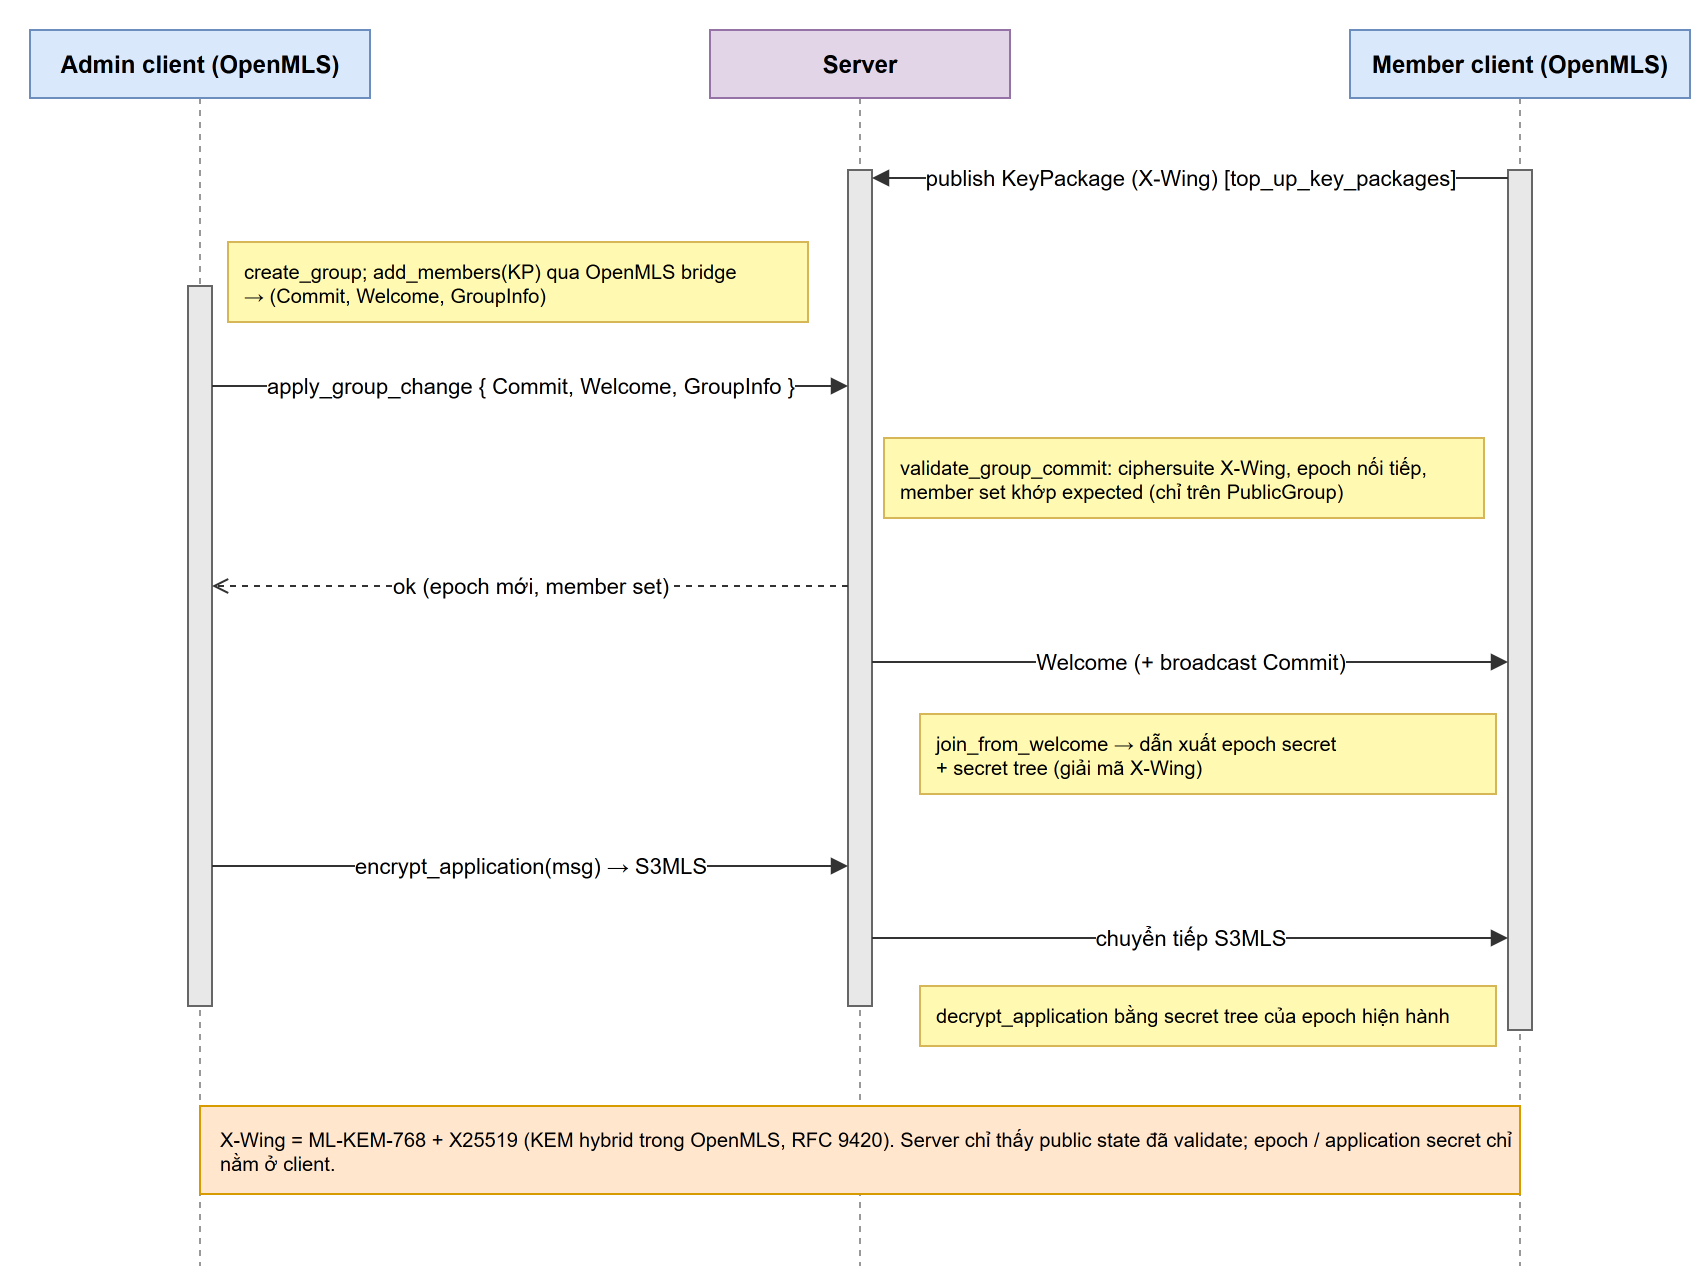
\includegraphics[width=0.92\linewidth]{Figure/SequenceMlsGroup.png}
    \caption{Sơ đồ tuần tự: vòng đời khóa group MLS X-Wing (KeyPackage $\rightarrow$ Commit/Welcome $\rightarrow$ epoch $\rightarrow$ application message)}
    \label{fig:seq-mls-group}
\end{figure}

Trạng thái verified trong DM không tự áp dụng cho group. Với group, client dựa vào MLS Welcome, Commit, GroupInfo, transcript checkpoint và kiểm tra identity từng thành viên để phát hiện state không nối tiếp hoặc lịch sử bị sắp xếp bất thường.

\begin{figure}[H]
    \centering
    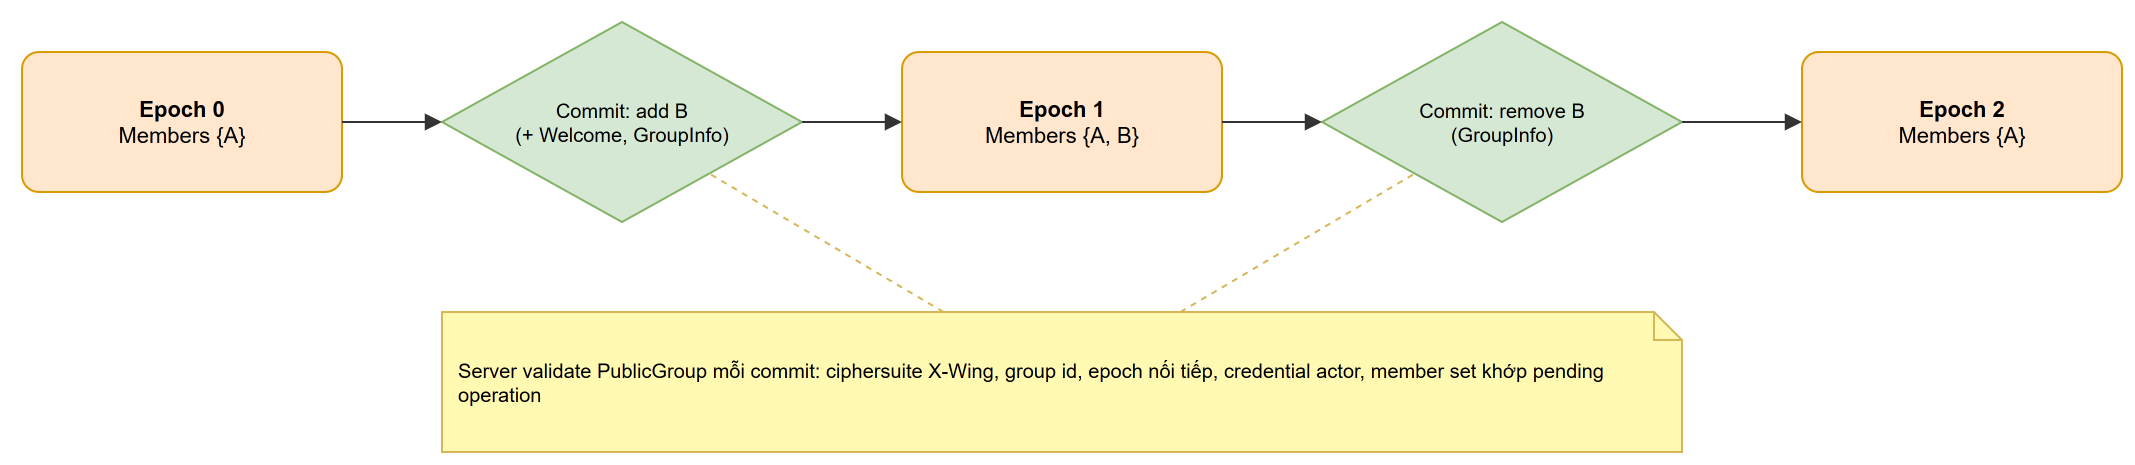
\includegraphics[width=0.9\linewidth]{Figure/GroupCommitChainFlow.png}
    \caption{Chuỗi MLS Commit dùng để kiểm tra thay đổi membership}
    \label{fig:groupcommitchainflow}
\end{figure}

Ngoài commit chain cho membership, client group còn có transcript checkpoint. Mỗi client tính hash nối tiếp trên các message đã chấp nhận, ký checkpoint bằng identity key và gửi checkpoint như một control message được mã hóa. Khi nhận checkpoint của thành viên khác, client so khớp với view cục bộ tại cùng message id. Nếu server bỏ sót message, đảo thứ tự hoặc cho hai client nhìn thấy history khác nhau, checkpoint có thể không khớp và UI sẽ có cơ sở để cảnh báo.

Khi có cảnh báo consistency, giao diện không chỉ ghi một dòng thông báo chung. Header hội thoại hiển thị trạng thái cảnh báo history và có nút Details để người dùng xem nội dung cụ thể của cảnh báo, ví dụ commit chain không nối tiếp, thiếu sự kiện membership hoặc transcript checkpoint không khớp. Cơ chế này không làm server mất khả năng gây từ chối dịch vụ, nhưng giúp client phát hiện và trình bày rõ hơn các trường hợp server trả view không nhất quán.

\begin{figure}[H]
    \centering
    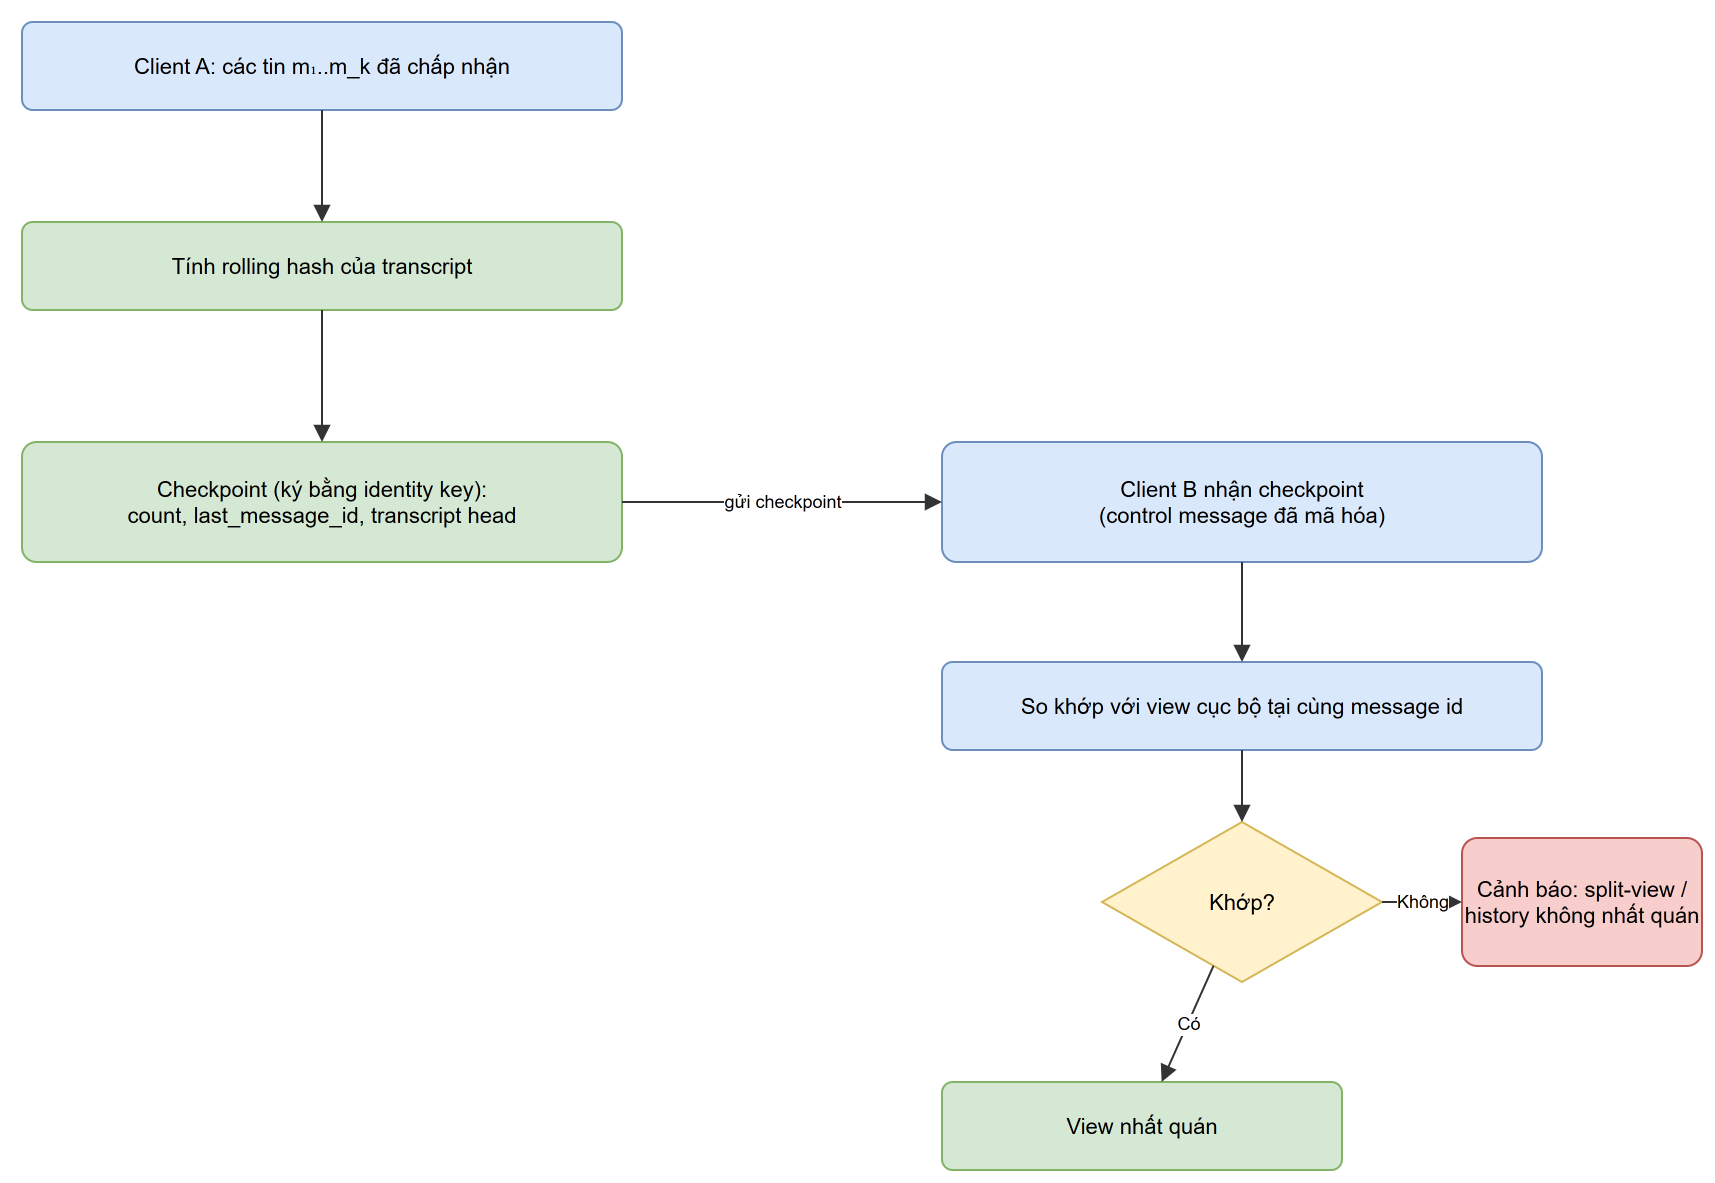
\includegraphics[width=0.9\linewidth]{Figure/TranscriptConsistencyFlow.png}
    \caption{Transcript checkpoint giúp phát hiện group history không nhất quán}
    \label{fig:transcriptconsistencyflow}
\end{figure}

\subsubsection{Local plaintext cache}

Vì Double Ratchet có tính forward secrecy, không phải mọi tin cũ đều có thể được giải mã lại vô hạn chỉ từ state hiện tại. Để trải nghiệm người dùng không bị mất lịch sử sau khi đăng xuất rồi đăng nhập lại, client lưu một cache plaintext cục bộ đã mã hóa bằng master key.

Đây là một đánh đổi có chủ ý. Cache giúp người dùng đọc lại lịch sử và giúp inbox preview hiển thị nội dung thật. Đổi lại, nếu attacker lấy được máy người dùng và mở được local state, lịch sử đã cache có thể bị đọc. Vì vậy UI có thiết lập bật hoặc tắt cache, thời gian giữ cache, xóa cache thủ công, xóa cache khi logout và tắt cache cho từng conversation nhạy cảm. Backup E2EE cũng phải cho người dùng chọn có đưa cache vào file backup hay không.

Cache được tách theo tài khoản và theo thư mục chạy của client, nên việc đổi sang tài khoản khác trên cùng thiết bị không được xóa cache của tài khoản cũ. Khi tài khoản cũ đăng nhập lại đúng thiết bị đó, các tin đã từng decrypt phải được lấy lại từ cache và hiển thị đúng thứ tự. Nếu một tài khoản mới được thêm vào group sau này, hoặc cùng tài khoản đăng nhập ở thiết bị khác chưa có cache, các ciphertext cũ không giải mã được sẽ bị ẩn khỏi UI thay vì hiện placeholder lỗi giải mã.

Backup E2EE là một snapshot do người dùng export và giữ bằng passphrase riêng, không phải cơ chế đồng bộ liên tục. Khi restore trên thiết bị mới, client giải mã snapshot, bọc lại bằng master key hiện tại, merge cache theo message id và công bố lại bundle mới dưới cùng identity nếu identity secret được khôi phục. Việc restore như vậy giúp khôi phục lịch sử đã có trong backup mà không làm thay đổi key của người đối thoại.

\begin{figure}[H]
    \centering
    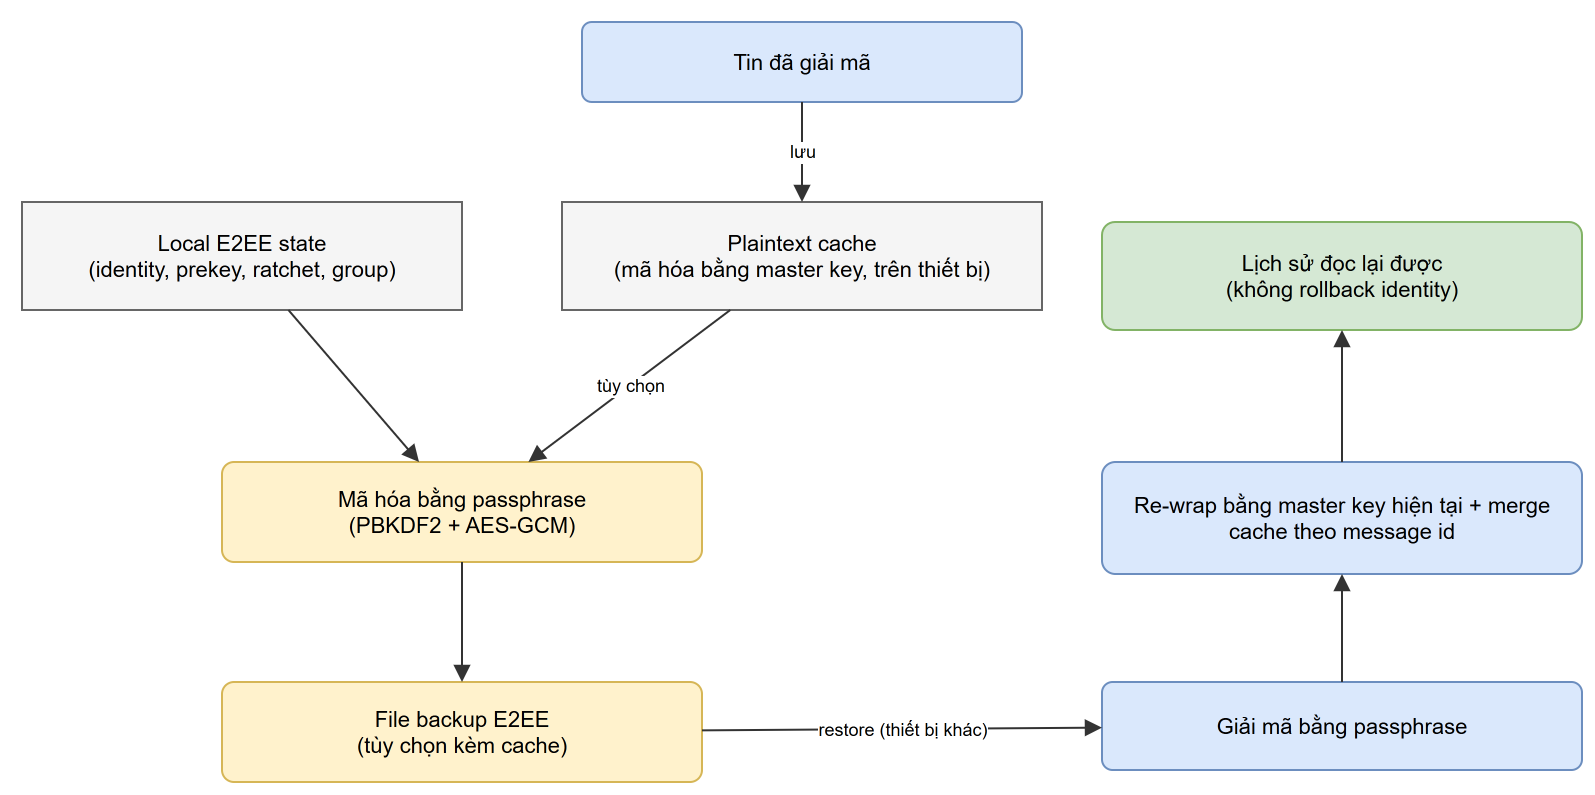
\includegraphics[width=0.9\linewidth]{Figure/CacheBackupFlow.png}
    \caption{Quan hệ giữa plaintext cache cục bộ và backup E2EE}
    \label{fig:cachebackupflow}
\end{figure}

\section{Thiết kế giao thức truyền tin}

\subsection{Các loại gói chính}

Các gói chính của giao thức được chia theo vai trò:
\begin{itemize}
    \item Nhóm xác thực gồm \texttt{register}, \texttt{auth} và \texttt{change\_password}.
    \item Nhóm hồ sơ gồm \texttt{get\_profile}, \texttt{update\_profile}, \texttt{upload\_avatar}, \texttt{remove\_avatar} và các lệnh privacy.
    \item Nhóm hội thoại gồm mở DM, tạo group, gửi message, tải history, lấy inbox và quản lý thành viên.
    \item Nhóm key gồm công bố identity, rotate identity, công bố PQXDH bundle, lấy PQXDH bundle và công bố MLS KeyPackage.
\end{itemize}

Các thay đổi membership dùng hai bước \texttt{prepare} và \texttt{apply}; chi tiết pending operation và validation public MLS state đã trình bày ở mục~\ref{subsubsec:group-mls}.

Nhóm message metadata xử lý pin, danh sách tin được ghim, reaction và typing indicator. Typing indicator có thể bị tắt vì đây là metadata nhạy cảm. Trạng thái unread chỉ áp dụng cho chính tài khoản hiện tại; hệ thống không gửi read receipt cho peer.

\subsection{Định dạng gói tin và quy trình đóng gói}\label{subsec:body-format}

Server chỉ chấp nhận message body có prefix E2EE hợp lệ. Với SecChat, các prefix chính là:

\begin{itemize}
    \item \texttt{S3PQI:} cho tin DM đầu tiên chứa transcript PQXDH-style.
    \item \texttt{S3DR:} cho tin DM sau khi đã vào Double Ratchet.
    \item \texttt{S3MLS:} cho tin group và encrypted group control message qua MLS.
\end{itemize}

Những prefix này là điều kiện bắt buộc để server lưu message mới. Nếu body không thuộc một trong ba dạng trên, server trả lỗi thay vì lưu dữ liệu, nhờ đó cơ sở dữ liệu không chứa plaintext message do client gửi nhầm.

\textbf{Quy trình đóng gói và mã hóa một tin DM.} Một tin nhắn trực tiếp được đóng gói ở client qua các bước sau trước khi rời thiết bị:
\begin{enumerate}
    \item Chuẩn bị plaintext. Nội dung văn bản được mã hóa UTF-8; nếu là tệp đính kèm thì client đặt một marker \texttt{FILE:} kèm dữ liệu tệp đã mã hóa base64 bên trong plaintext, nên với giao thức mọi tin đều là một khối plaintext thuần nhất.
    \item Lấy khóa và dựng header. Double Ratchet tiến chain key gửi để sinh một message key dùng một lần, đồng thời dựng header gồm khóa ratchet công khai hiện hành, số thứ tự tin và độ dài chain trước.
    \item Mã hóa có xác thực (AEAD). Plaintext được mã hóa bằng message key với header làm dữ liệu xác thực kèm theo (AAD), cho ra ciphertext và một thẻ xác thực; thẻ này ràng buộc cả header lẫn nội dung nên mọi sửa đổi đều bị phát hiện khi giải mã.
    \item Gắn prefix và đóng khung. Header, ciphertext và thẻ được nối lại, biểu diễn ở dạng văn bản base64 rồi gắn prefix \texttt{S3DR:} (riêng tin đầu phiên dùng \texttt{S3PQI:} và đính kèm transcript bắt tay PQXDH để phía nhận tái lập root secret).
    \item Bọc trong bản tin JSON và gửi qua TLS. Chuỗi có prefix được đặt vào trường \texttt{body} của một bản tin JSON; các trường định tuyến như mã hội thoại, người gửi và thời điểm vẫn ở dạng rõ để server xử lý. Bản tin JSON được gửi trong một khung WebSocket nằm trong kênh TLS.
\end{enumerate}
Ở phía server, sau khi kiểm tra quyền và prefix hợp lệ, toàn bộ trường \texttt{body} (ciphertext) được lưu nguyên văn vào bảng \texttt{messages} và chuyển tiếp; server không hề giải mã. Phía nhận làm ngược lại: tách prefix, giải mã base64, tách header, tiến hoặc xoay ratchet để lấy đúng message key, rồi giải mã và kiểm tra thẻ AEAD trên cả header lẫn ciphertext; nếu thẻ không hợp lệ thì tin bị loại bỏ. Tin nhóm theo cùng nguyên tắc nhưng dùng lớp mã hóa application message của MLS (khóa lấy từ secret tree của epoch) và mang prefix \texttt{S3MLS:}.

Khác với một giao thức đường hầm có bố cục nhị phân cố định, gói tin SecChat là một envelope JSON được mã hóa base64 nên độ dài thay đổi theo nội dung; tuy vậy các thành phần mật mã bên trong đều có kích thước cố định. Với một tin DM (\texttt{S3DR}), các trường quan trọng và kích thước của chúng gồm:
\begin{itemize}
    \item Prefix \texttt{S3DR:} -- 5 byte ASCII, là điều kiện để server chấp nhận lưu.
    \item \texttt{sid} -- định danh phiên ngẫu nhiên 16 byte.
    \item \texttt{h} (header, đồng thời là AAD): khóa công khai ratchet X25519 \texttt{dh} 32 byte, hai bộ đếm \texttt{pn}/\texttt{n}, và các trường định tuyến \texttt{conversation\_id}, \texttt{sender\_uid}, \texttt{recipient\_uid}, \texttt{sender\_identity\_version}.
    \item \texttt{ct} -- kết quả AES-256-GCM gồm nonce 12 byte $\Vert$ ciphertext (dài bằng plaintext) $\Vert$ thẻ xác thực 16 byte; khóa là message key 32 byte do Double Ratchet sinh.
    \item \texttt{eh} -- một bản sao header được mã hóa thêm bằng header key để giấu metadata ratchet.
\end{itemize}
Riêng tin mở phiên (\texttt{S3PQI}) mang thêm transcript bắt tay PQXDH: khóa định danh Ed25519 32 byte, signed prekey X25519 32 byte kèm chữ ký Ed25519 64 byte, một khóa ephemeral X25519 32 byte và ciphertext ML-KEM-1024 dài 1568 byte. Toàn bộ cấu trúc gói tin cùng hành trình mã hóa -- truyền -- giải mã được tổng hợp ở Hình~\ref{fig:packet-format}.

\begin{figure}[H]
    \centering
    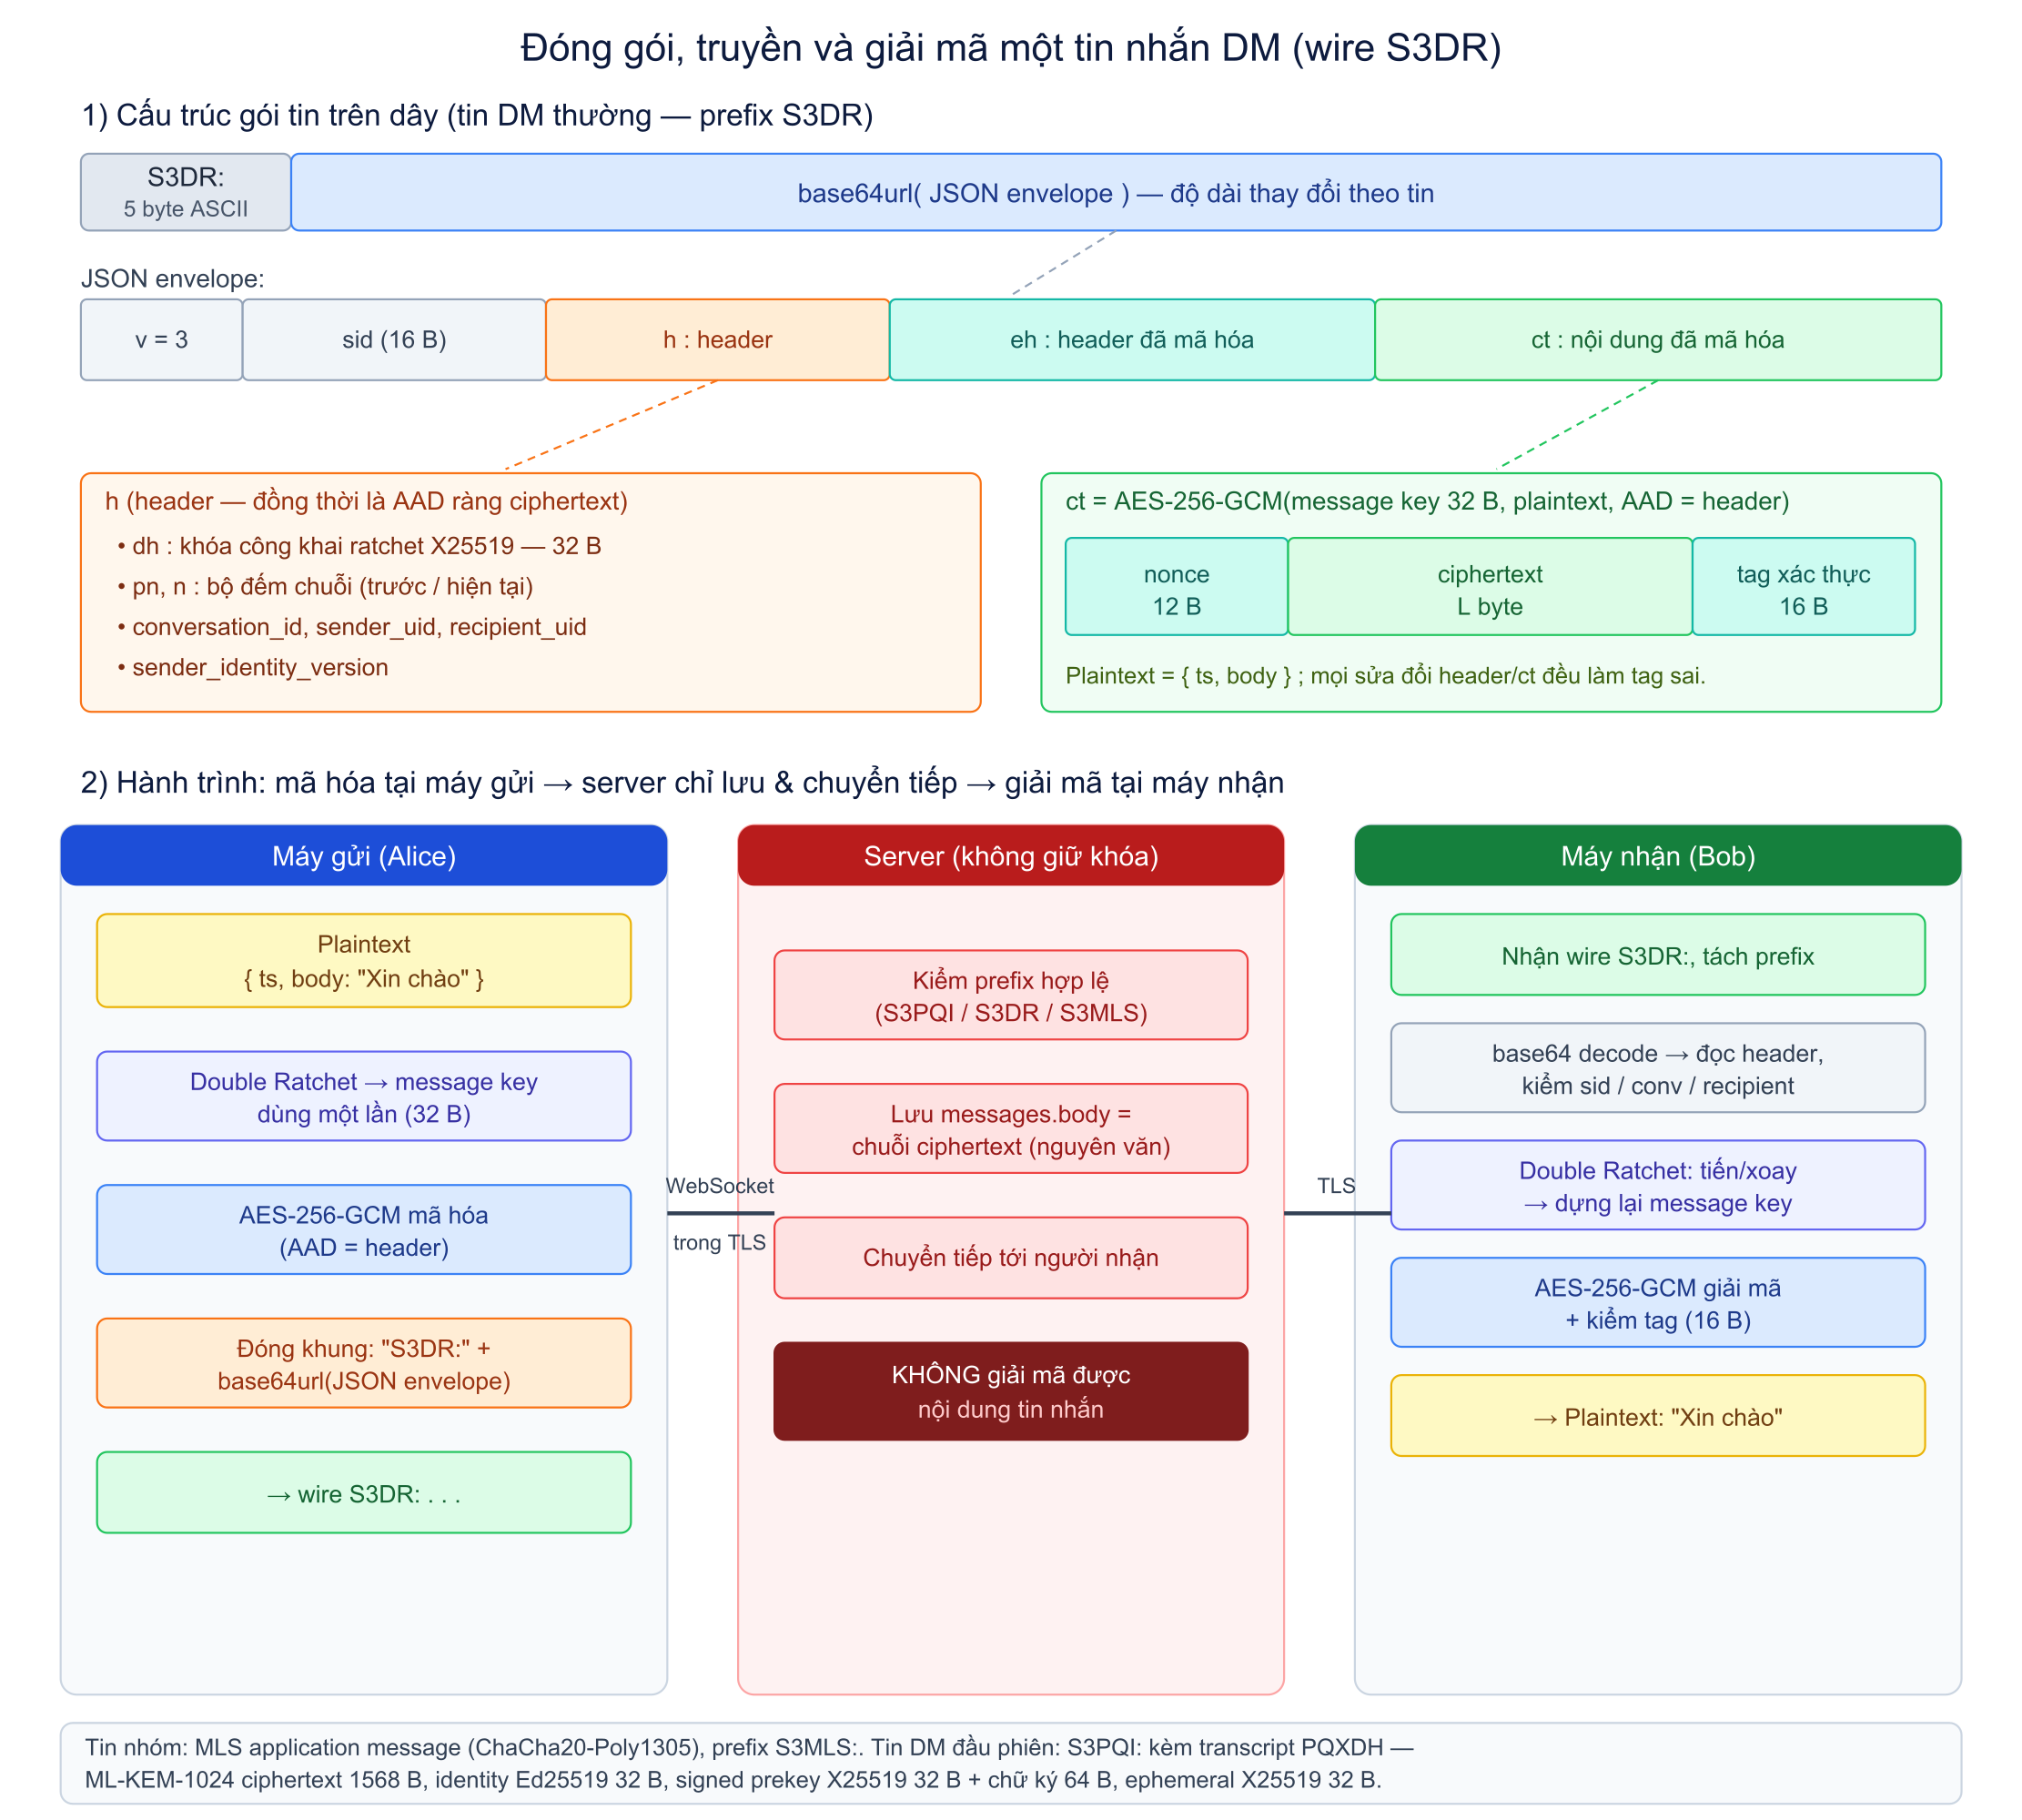
\includegraphics[width=\linewidth]{Figure/MessagePacketFormat.png}
    \caption{Cấu trúc gói tin S3DR và hành trình đóng gói, truyền, giải mã một tin DM}
    \label{fig:packet-format}
\end{figure}

\begin{figure}[H]
    \centering
    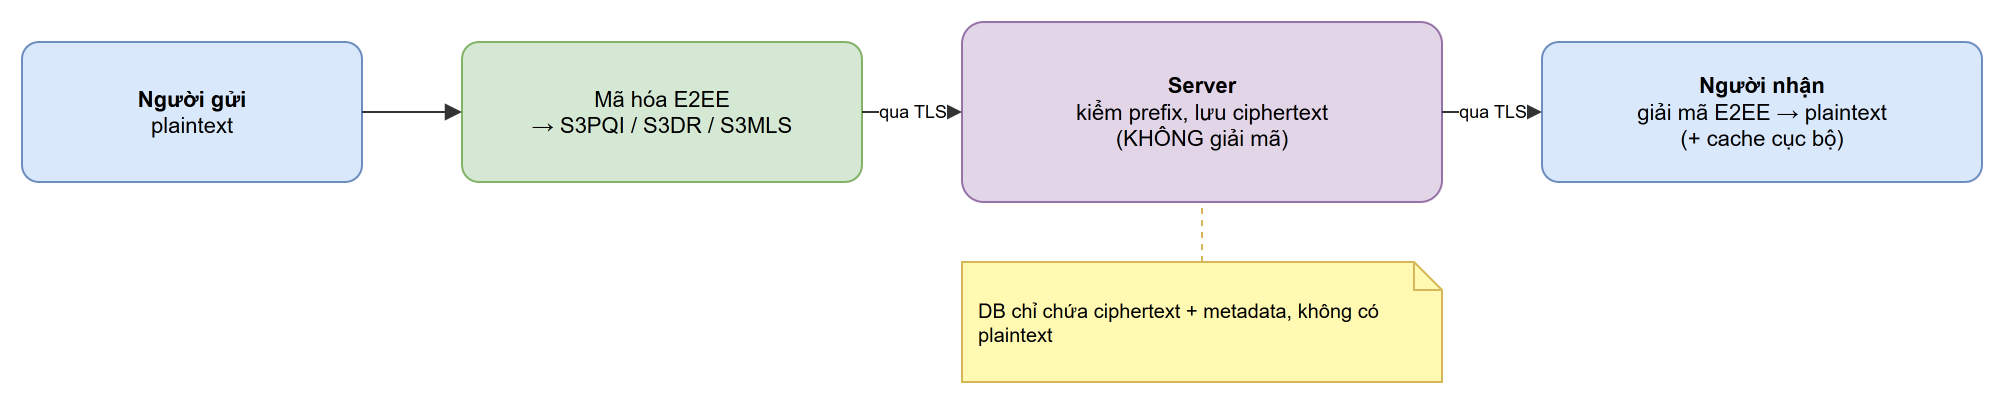
\includegraphics[width=0.9\linewidth]{Figure/MessageDataFlow.png}
    \caption{Data flow của một tin nhắn đã mã hóa đầu cuối}
    \label{fig:messagedataflow}
\end{figure}

\subsection{Metadata và quyền riêng tư}

Theo mô hình tin cậy ở mục~\ref{sec:security-protocol}, hệ thống chỉ bảo vệ nội dung tin nhắn, còn metadata vẫn nằm trong phạm vi tin cậy của server. Server cần metadata để vận hành inbox, group membership, history, pin, reaction và trạng thái unread cục bộ. Đây là giới hạn quan trọng của thiết kế và được đánh giá kỹ hơn ở chương thực nghiệm.

\section{Thiết kế client}

\subsection{Tổ chức mã nguồn}

Client được chia thành các phần chính. \texttt{client/pages} chứa các trang giao diện như đăng nhập, đăng ký và chat. \texttt{client/network.py} quản lý kết nối WebSocket qua TLS. \texttt{client/dialogs.py} chứa các dialog hồ sơ, avatar, đổi mật khẩu và thiết lập phụ. \texttt{client/crypto\_engine} chứa phần giao thức và trạng thái crypto.

Package \texttt{client/crypto\_engine} chứa primitive của giao thức như tạo bundle, kiểm tra chữ ký prekey, transcript kiểu PQXDH, Double Ratchet và wrapper OpenMLS. \texttt{client/crypto\_engine/openmls\_bridge.py} gọi bridge Rust dùng ciphersuite X-Wing. \texttt{client/crypto\_engine/session.py} quản lý state của phiên người dùng, file key mã hóa, cache plaintext mã hóa, trạng thái ratchet, trạng thái MLS group và mã hóa tin gửi đi.

\begin{figure}[H]
    \centering
    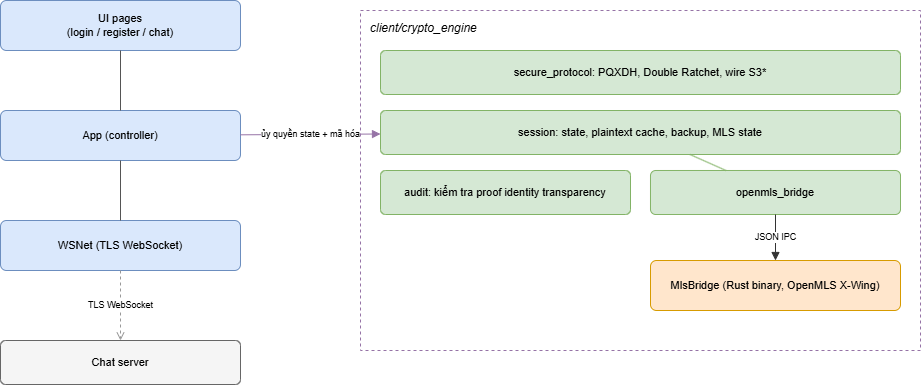
\includegraphics[width=0.9\linewidth]{Figure/CryptoEngineSplit.png}
    \caption{Ranh giới giữa UI controller và crypto engine}
    \label{fig:cryptoenginesplit}
\end{figure}

\subsection{Vai trò của App}

\texttt{client/app.py} là controller chính của ứng dụng PyQt. Nó nhận tín hiệu từ UI, gửi lệnh qua WebSocket, nhận event từ server và cập nhật giao diện. Controller này không sở hữu trực tiếp toàn bộ crypto state; các thao tác như lưu identity key, lưu prekey, lưu ratchet state, lưu group state, cache message, rotate identity và encrypt outbound message được ủy quyền cho \texttt{CryptoSession}.

Một phần decrypt message nhận vào và replay history vẫn được \texttt{App} điều phối cùng \texttt{CryptoSession}. Cách tổ chức này giữ UI controller ở vai trò phối hợp sự kiện, còn state nhạy cảm vẫn thuộc crypto engine.

\subsection{Giao diện chat}

UI hỗ trợ các thao tác quen thuộc của ứng dụng chat: danh sách hội thoại, friend list, avatar, profile, đổi mật khẩu, privacy, block, typing indicator, reaction, pin và forward. Read receipt không nằm trong UI; trạng thái read/unread chỉ phục vụ quản lý inbox cục bộ. Các hành động trên từng tin nhắn được gom vào nút ba chấm để tránh làm rối vùng timestamp. Forward hiển thị nhãn nhỏ, edit hiển thị trạng thái đã sửa, reaction hiển thị chip dưới tin nhắn, còn tin được ghim có badge và xuất hiện trong danh sách Pins.

Message view dùng \texttt{MessageListView} dựa trên \texttt{QScrollArea}, trong đó mỗi message là một row widget có layout riêng. Cách này phù hợp với các thao tác như menu ba chấm, reaction chip, badge pin, drag-drop file và trạng thái gửi.

\section{Thiết kế server}

\subsection{Kiến trúc phân tầng}

Server C được tách thành các lớp rõ ràng. \texttt{transport} xử lý socket, WebSocket, danh sách client và HTTP control plane. \texttt{protocol} xử lý JSON. \texttt{infra} chứa cấu hình, log, crypto helper, metrics, database pool, migration và rate limit. \texttt{domain} chứa validation. \texttt{repository} chứa truy vấn SQL. \texttt{services} chứa logic nghiệp vụ: auth, messaging, groups, keys, friends, profile, presence, blocking, notifications, reaction, pin, disappearing và conversation preferences (cùng dispatcher \texttt{chat}).

Việc tách lớp giúp \texttt{main.c} không phình thành một file chứa mọi nghiệp vụ. Khi có lệnh mới, service tương ứng xử lý qua dispatcher riêng, còn repository chịu trách nhiệm truy cập database bằng prepared statement.

\subsection{Xác thực, rate limit và đổi mật khẩu}

Cơ chế băm mật khẩu hai tầng client–server và dẫn xuất master key đã trình bày ở mục~\ref{subsubsec:password}. Ở góc độ server, điểm cần nhấn mạnh là server chỉ thao tác trên hash nhận từ client nên không bao giờ thấy mật khẩu gốc; khi đổi mật khẩu, server kiểm tra hash cũ rồi lưu hash mới, còn việc bọc lại local E2EE state bằng master key mới do client tự thực hiện. Nếu mật khẩu sai, server trả lỗi để UI báo rõ là email hoặc mật khẩu không đúng.

Rate limit được áp dụng cho luồng xác thực để giảm rủi ro brute-force. Log không nên ghi trực tiếp email hoặc dữ liệu nhạy cảm.

\subsection{Lưu và chuyển tiếp message}

Khi nhận message, server kiểm tra người gửi có quyền trong conversation và body có prefix E2EE hợp lệ (mục~\ref{subsec:body-format}), nhưng không giải mã message. Sau khi lưu vào bảng \texttt{messages}, server phát event cho các thành viên đang online; nếu người nhận offline, message vẫn nằm trong lịch sử và inbox giúp client tải lại khi người đó đăng nhập. Riêng edit message được lưu theo hướng event-sourced - thêm một row event trỏ về tin gốc qua \texttt{edit\_target\_message\_id} thay vì ghi đè ciphertext cũ - nhờ đó bản gốc không bị mất.

\subsection{Group và MLS validation}

Quy trình hai bước \texttt{prepare}/\texttt{apply} cùng các kiểm tra của MLS validator trên \texttt{PublicGroup} đã được mô tả ở mục~\ref{subsubsec:group-mls}. Ở góc độ server, điểm cần nhấn mạnh là server không bao giờ chỉ nhận base64 artifact rồi cập nhật thẳng bảng thành viên: mọi thay đổi membership chỉ được ghi sau khi validation pass, ngược lại handshake không được lưu và membership giữ nguyên. Vì chỉ làm việc trên public state, server có đủ dữ liệu để từ chối Commit giả mạo hoặc nằm ngoài policy nhưng không có application secret để đọc nội dung group. Các artifact MLS đã validate được lưu để thành viên replay Welcome/Commit đúng thứ tự khi online lại hoặc tải lại history.

\subsection{Vận hành và giám sát}

Server có HTTP control plane để trả health, readiness và metrics. Server GUI dùng dữ liệu này để hiển thị trạng thái vận hành qua các tab cần thiết như logs và metrics.

